\documentclass{article}

\PassOptionsToPackage{numbers, compress}{natbib} 
% 카톡으로 말한거 - 참조 숫자로하는거


\usepackage{amssymb}% http://ctan.org/pkg/amssymb
\usepackage{pifont}% http://ctan.org/pkg/pifont

\usepackage{graphicx} % Required for inserting images
\usepackage{wrapfig}
\usepackage{booktabs}   % \toprule, \midrule, \cmidrule, \bottomrule
\usepackage{multirow}   % \multirow
\usepackage{graphicx}   % \rotatebox, \resizebox
\usepackage{amsmath}
\usepackage{amssymb}
\usepackage{algorithm}
\usepackage{algpseudocode}
\usepackage{neurips_2026}
\usepackage{pdflscape}
\usepackage{adjustbox}
\usepackage[utf8]{inputenc} % allow utf-8 input
\usepackage[T1]{fontenc}    % use 8-bit T1 fonts
\usepackage{hyperref}       % hyperlinks
\usepackage{url}            % simple URL typesetting
\usepackage{booktabs}       % professional-quality tables
\usepackage{amsfonts}       % blackboard math symbols
\usepackage{nicefrac}       % compact symbols for 1/2, etc.
\usepackage{microtype}      % microtypography
\usepackage{xcolor}         % colors
\usepackage{kotex}
\usepackage{array}
\newcommand\jh[1]{\textcolor{red}{#1}}
\newcommand{\cmark}{\ding{51}}%
\newcommand{\xmark}{\ding{55}}


\usepackage{booktabs}
\usepackage[table]{xcolor}

\title{GRIK: Grouped Relevance-Integrated Key Cache Pruning for Grouped-Query Attention LLMs}

\begin{document}

\maketitle

\begin{abstract}
The key–value (KV) cache is a dominant memory bottleneck in long-context inference for large language models. Grouped-query attention (GQA), now adopted as the de facto standard in widely deployed models such as LLaMA-3, Mistral, and Qwen, structurally reduces KV storage, and compression methods must respect this architectural design to preserve its benefit. Existing channel-pruning methods, however, derive pruning masks at the query-head granularity and thereby violate the shared-KV storage model of GQA—inflating rather than reducing the realized cache footprint. We present GRIK, a training- and calibration-free channel-pruning method for the K cache that preserves GQA storage by construction. Our method aggregates the influence of query heads within each group through their output-projection contributions to derive a KV-head-shared mask, and prunes channels progressively toward the target ratio under a score that combines the K-projection weight norm with attention energy. On LLaMA-3-8B with 60\% channel retention, GRIK matches or surpasses the strongest prior channel-pruning method across a majority of LongBench tasks while reducing the realized K-cache footprint to $0.60\times$ Full~KV; in contrast, ThinK inflates the K cache to $\sim\!3.2\times$ under GQA storage and SparK leaves the footprint unchanged at $1.00\times$. Combined with FP8 KV quantization, the realized K-cache footprint reaches $0.30\times$ the bf16 baseline, a more than $3\times$ saving without retraining or calibration. Because all masks are determined dynamically per prompt, the method applies out of the box under varying compression ratios and across model checkpoints, with no recalibration required.
\end{abstract}


\section{Introduction}
\label{sec:intro}
Large language models (LLMs) have achieved strong performance across a wide range of real-world applications, but this progress has introduced a growing systems challenge: modern deployment increasingly requires long-context inference at scale. In autoregressive decoding, the dominant bottleneck is often no longer model parameters, but the key-value (KV) cache, which stores token-wise representations to avoid recomputation across decoding steps. Although essential for efficient generation, the KV cache grows linearly with both context length and batch size, and can quickly exceed the memory footprint of the model weights themselves. For Llama-3-8B, for example, the KV cache reaches 128\,GiB at sequence length 32K and batch size 32, roughly \(8\times\) the model's weight size and beyond the capacity of a single A100 GPU. Thus, the practical scalability of long-context LLMs is increasingly constrained by runtime KV memory rather than by model size alone.


\begin{figure}[t]
\centering
\begin{minipage}[t]{0.49\linewidth}
    \centering
    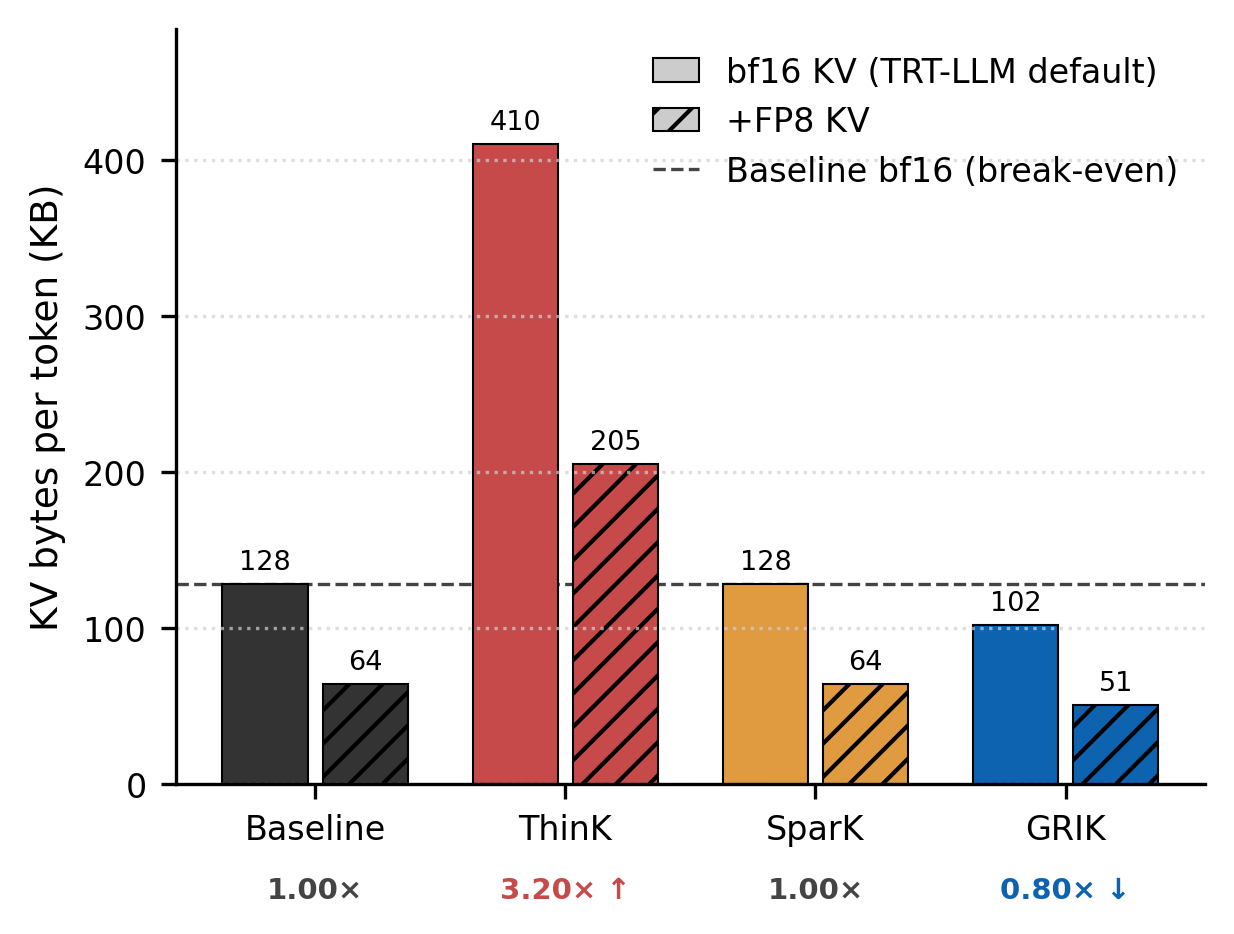
\includegraphics[width=\linewidth]{figs/motivation1.png}\\[2pt]
    {\small \textbf{(a)} Per-token KV memory.}
\end{minipage}\hfill
\begin{minipage}[t]{0.49\linewidth}
    \centering
    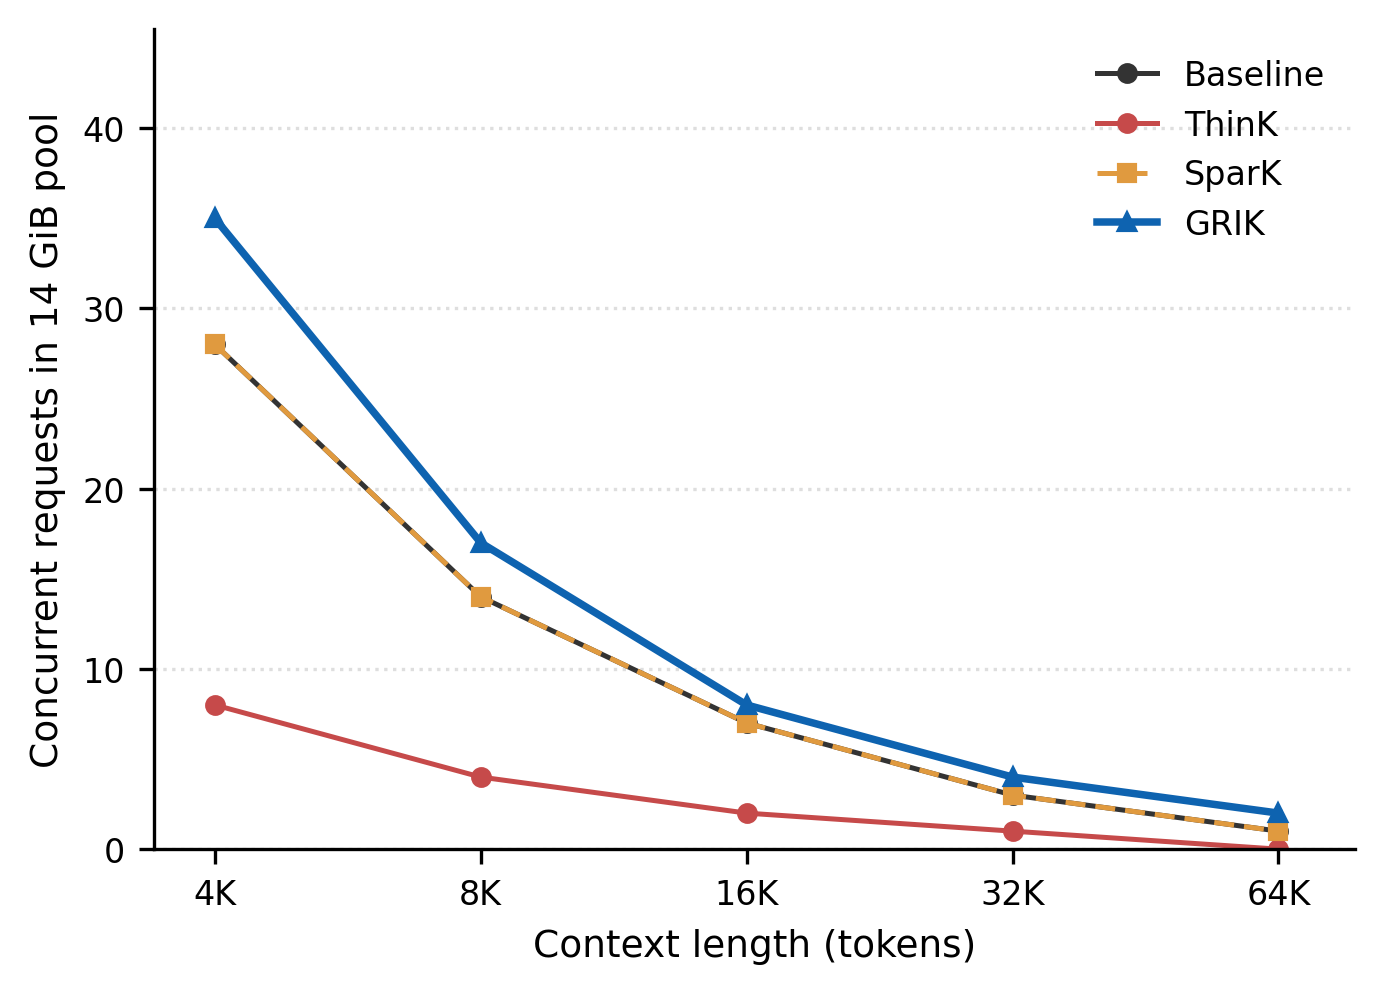
\includegraphics[width=\linewidth]{figs/motivation2.png}\\[2pt]
    {\small \textbf{(b)} Concurrent capacity in a 14~GiB pool.}
\end{minipage}
\caption{\textbf{The structural problem is operational on both axes.} \textbf{(a)} Per-token KV-cache memory at $r{=}0.4$ (LLaMA-3-8B, K+V in fp16 and FP8): GRIK $0.80\times$, ThinK $3.20\times$, SparK $1.00\times$. \textbf{(b)} Concurrent sequences fitting a $14$~GiB KV pool vs.\ context length.}
\label{fig:teaser}
\end{figure}


% Recent efficient LLMs have widely adopted grouped-query attention (GQA) to alleviate this bottleneck. In GQA, \(H\) query heads are mapped to \(H_{kv}\) shared key-value heads, reducing per-token KV storage from \(H \cdot d\) to \(H_{kv} \cdot d\). However, this gain is only partial: GQA removes redundancy across heads, but leaves the channel dimension \(d\) within each retained KV head untouched. As a result, KV memory still grows linearly with sequence length, making channel-level compression the next natural target. 

Recent efficient LLMs have widely adopted grouped-query attention (GQA) to alleviate this bottleneck. In GQA, \(H\) query heads are mapped to \(H_{kv}\) shared key-value heads, reducing per-token KV storage from \(H \cdot d\) to \(H_{kv} \cdot d\). However, this gain is only partial: GQA removes redundancy across heads, but leaves the channel dimension \(d\) within each retained KV head untouched. As a result, KV memory still grows linearly with sequence length, making channel-level compression the next natural target. Yet this residual cost cannot be reduced by arbitrary dimension pruning. Because GQA stores a shared K/V tensor at KV-head granularity, any downstream channel-pruning scheme must use masks that are both KV-head-aligned and token-consistent; otherwise, dimensions may be nominally pruned without reducing the underlying cache footprint. Existing KV-dimension pruning methods do not explicitly account for this GQA storage constraint, and therefore fail to translate dimension sparsity into actual cache reduction. The remaining challenge is therefore structural rather than merely statistical.


To address this gap, we propose \textbf{GRIK} (Grouped Relevance-Integrated Key pruning), a GQA-compatible channel-pruning method that preserves shared-KV storage \emph{by construction}. The key idea is that, under GQA, channel sparsity leads to actual cache reduction only when the pruning mask is both KV-head-aligned and token-consistent. GRIK enforces exactly this structure by assigning a single shared mask to each KV head, yielding a pruned dense cache of shape \(\mathbb{R}^{H_{kv} \times T \times \lfloor r d \rfloor}\) at retention ratio \(r\).

This view also clarifies why channel pruning is complementary to existing KV-efficiency strategies. Token eviction reduces memory by discarding entire token states, but may irreversibly remove information needed later in long-context reasoning. Quantization lowers numerical precision, but preserves tensor dimensionality and therefore does not reduce the number of stored features. Channel pruning instead preserves all tokens while reducing the representational budget of each token, directly targeting the residual per-head memory cost left untouched by GQA.

Existing channel-pruning methods violate the structural requirement above in different ways. ThinK~\citep{think} uses query-head-specific masks, which break consistency within a shared GQA group and effectively forfeit the storage efficiency gained by GQA. SparK~\citep{spark} uses token-wise unstructured masks, so different tokens retain different channel subsets, which precludes tensor-shape reduction in principle. As a result, although both methods nominally prune key dimensions, neither yields an actual reduction in GQA cache footprint (Figure~\ref{fig:teaser}). By contrast, GRIK aggregates channel-selection signals from all query heads within each KV group into a single shared mask, combining a static prior from the K-projection row norm with a prompt-specific dynamic signal from attention energy. It requires neither training nor offline calibration, and physically reduces the cached K tensor at prefill time. Across LongBench~\citep{longbench} and RULER~\citep{ruler}, GRIK at $60\%$ channel retention matches or exceeds ThinK and SparK on the majority of tasks while reducing the realized K-cache footprint to $0.60\times$ the uncompressed baseline, in contrast to ThinK's $\sim\!3.2\times$ inflation under GQA storage and SparK's unchanged footprint.

% The main obstacle, however, is structural rather than statistical. Because GQA stores a shared K/V tensor at KV-head granularity, any downstream channel-pruning scheme must use masks that are both KV-head-aligned and token-consistent. Existing methods violate this requirement in different ways. ThinK uses query-head-specific masks, which break consistency within a shared GQA group and effectively forfeit the storage efficiency gained by GQA. SparK uses token-wise unstructured masks, so different tokens retain different channel subsets, which precludes tensor-shape reduction in principle. As a result, although both methods nominally prune key dimensions, neither yields an actual reduction in GQA cache footprint. By contrast, GRIK aggregates channel-selection signals from all query heads within each KV group into a single shared mask, combining a static prior from the K-projection row norm with a prompt-specific dynamic signal from attention energy. It requires neither training nor offline calibration, and physically reduces the cached K tensor at prefill time. Across LongBench, RULER, and GSM-Infinite, GRIK at 60\% channel retention matches or exceeds ThinK and SparK on the majority of tasks while reducing actual K-cache memory to \(0.60\times\) the uncompressed baseline, in contrast to ThinK's \(3.4\times\) inflation and SparK's unchanged footprint.
%%%%%%%%%%%%%%%%%%%%%%%%%%%%%%%%%%%%%%%%%%%%%%%%%
% Large language models (LLMs) have achieved remarkable success across a wide range of real-world applications, but this progress has also introduced a growing systems challenge: modern deployment increasingly demands long-context inference at scale. In autoregressive decoding, the dominant bottleneck in this regime is often no longer model parameters, but the key-value (KV) cache, which stores token-wise representations to avoid recomputation across decoding steps. Although indispensable for efficient generation, the KV cache grows linearly with both context length and batch size, and can quickly exceed the memory footprint of the model weights themselves. For Llama-3-8B, for example, the KV cache reaches 128\,GiB at sequence length 32K and batch size 32, roughly \(8\times\) the model's weight size and beyond the capacity of a single A100 GPU. As a result, the practical scalability of long-context LLMs is increasingly constrained not by model size alone, but by the runtime memory cost of cached activations.

% Recent efficient LLMs have widely adopted grouped-query attention (GQA) to alleviate this bottleneck. In GQA, \(H\) query heads are mapped to \(H_{kv}\) shared key-value heads, so that each KV head is shared by \(g = H/H_{kv}\) query heads. For an input sequence of length \(T\), the key cache of each layer is therefore stored as \(K \in \mathbb{R}^{H_{kv} \times T \times d}\), where \(d\) denotes the head dimension. This reduces per-token KV storage from \(H \cdot d\) to \(H_{kv} \cdot d\). Yet this architectural gain is only partial: while GQA removes redundancy across heads, it leaves the channel dimension \(d\) within each retained KV head untouched. Consequently, even in GQA-based models, KV memory still grows linearly with sequence length, making the residual per-head channel dimension the next natural target for compression.

% To address this gap, we propose \textbf{GRIK} (Grouped Relevance-Integrated Key pruning), a GQA-compatible channel-pruning method that preserves shared-KV storage \emph{by construction}. The central idea is simple: under GQA, channel sparsity leads to actual cache reduction only when the pruning mask is aligned with the KV-head storage layout and remains consistent across tokens. GRIK enforces exactly this structure by assigning a single shared mask to each KV head, rather than using query-head-specific or token-specific masks. With a retention ratio \(r\), this directly yields a pruned dense cache of shape \(\mathbb{R}^{H_{kv} \times T \times \lfloor r d \rfloor}\), translating logical channel sparsity into physical cache reduction.

% This perspective makes channel-level compression a natural complement to existing KV-efficiency strategies. Token eviction reduces memory by discarding entire token states, but may irreversibly remove information that becomes important later in long-context reasoning. Quantization lowers numerical precision, but preserves tensor dimensionality and therefore does not reduce the number of stored features. Channel pruning occupies a distinct and complementary point in this design space: it preserves all tokens while reducing the representational budget of each token. In modern GQA-based LLMs, this directly targets the residual per-head memory cost left untouched by head sharing.

% The main obstacle, however, is structural rather than statistical. Because GQA stores a shared K/V tensor at KV-head granularity, any downstream channel-pruning scheme must use masks that are both KV-head-aligned and token-consistent. Existing methods violate this requirement in different ways. ThinK applies query-head-specific masks, which break consistency within a shared GQA group and effectively forfeit the storage efficiency gained by GQA. SparK applies token-wise unstructured masks, so different tokens retain different channel subsets, which precludes tensor-shape reduction in principle. As a result, although both methods nominally prune key dimensions, neither yields an actual reduction in GQA cache footprint. On LLaMA-3-8B with 60\% channel retention, ThinK inflates K-cache memory to \(3.4\times\) the uncompressed GQA baseline, while SparK leaves the footprint unchanged. Better scoring alone cannot resolve this issue, because the mismatch lies in mask granularity itself.

% GRIK is designed around this structural insight. It aggregates the channel-selection contributions of all query heads within each KV group into a single shared mask, weighted by each head's output-projection influence so that heads with larger impact on the residual stream drive the decision. Its channel score combines two complementary signals: a data-independent static prior from the row norm of the K projection, and a prompt-specific dynamic signal from the attention energy induced by the current input. Channels are removed progressively toward the target retention ratio, with the mask and the resulting attention distribution refined jointly at each step. Because all statistics are computed from the prompt at prefill time, GRIK requires neither training nor offline calibration, and physically reduces the cached K tensor to \(H_{kv} \cdot T \cdot \lfloor r d \rfloor\). Across LongBench, RULER, and GSM-Infinite, GRIK at 60\% channel retention matches or exceeds the accuracy of ThinK and SparK on the majority of tasks while reducing actual K-cache memory to \(0.60\times\) the uncompressed baseline, in contrast to ThinK's \(3.4\times\) inflation and SparK's unchanged footprint.

%%%%%%%%%%%%%%%%%%%%%%%%%%%%%%%%%%%%%%%%%%%%%%%%%%%%%%%%%%%

% Large language models now routinely process inputs of tens of thousands of tokens, and long-context inference has become a central deployment scenario. The key-value (KV) cache, which stores per-token representations to avoid recomputation during autoregressive decoding, has emerged as the dominant memory bottleneck in this regime~\citep{pope2023efficient}. Its size grows linearly with both sequence length and batch size, quickly surpassing the footprint of the model weights themselves. At sequence length 32K and batch size 32, the KV cache of LLaMA-3-8B~\citep{llama3} reaches 128~GiB, roughly eight times its weight size and exceeding the capacity of a single NVIDIA A100. Efficient KV cache compression is therefore essential for realizing the long-context capabilities that modern LLMs nominally support.

% Prior work organizes along three orthogonal axes. The \emph{token} axis removes tokens deemed less important for generation~\citep{h2o, snapkv, adakv}, while \emph{quantization} reduces the numerical precision of stored values~\citep{kivi, kvquant}. The \emph{channel} axis, which this paper studies, removes dimensions within each token's key vector. Despite being the axis most directly tied to the design of the attention module, it has received comparatively little attention. The two representative prior works, ThinK~\citep{think} and SparK~\citep{spark}, are both structurally misaligned with the attention architecture of modern LLMs, in two different ways.

% Modern LLMs have widely adopted grouped-query attention (GQA)~\citep{gqa} as their standard architecture. GQA lets multiple query heads within a group share a single set of key and value vectors, reducing per-token KV storage from $H \cdot d$ to $H_{kv} \cdot d$. Preserving this architectural gain imposes a strict requirement on any downstream compression method: pruning masks on the K cache must be defined at \emph{KV-head} granularity and must remain consistent across tokens. Existing channel-pruning methods, however, violate this condition in two distinct ways. ThinK applies a per-query-head mask, which differs within each GQA group and therefore makes single-tensor storage at $H_{kv}$-head granularity impossible; the cache falls back to $H$-head storage and its memory footprint grows rather than shrinks. SparK applies a per-token unstructured mask, which retains a different subset of channels for each token and rules out any tensor-shape reduction in principle; in the open-source implementation, the tensor keeps its original size and the dropped channels are overwritten by stochastic samples. Measured on LLaMA-3-8B at 60\% channel retention, ThinK consumes $3.4\times$ the K-cache memory of the uncompressed GQA baseline, while SparK matches it exactly (Figure~\ref{fig:teaser}). Each K vector is nominally compressed, yet the cache does not shrink. No refinement of the scoring function can resolve this; the mismatch is structural.

% The same tension between GQA's shared-KV structure and head-wise compression has been observed indirectly along other axes, both in token eviction~\citep{adakv} and in query-aware sparse attention~\citep{twilight}. On the channel axis, however, it has not been addressed systematically, and existing methods retain either query-head or per-token mask granularity. We close this gap by redefining the granularity of the mask decision itself: a single shared mask per KV-head group, consistent across tokens and applied as a structured reduction of the K tensor.

% We propose \textbf{GRIK} (Grouped Relevance-Integrated Key pruning), a training-free, calibration-free channel-pruning method that preserves GQA storage \emph{by construction}. GRIK aggregates the channel-selection contributions of all query heads within each KV group into a single shared mask, weighted by each head's \emph{output-projection influence} so that heads with larger effect on the residual stream drive the decision. The channel score combines two complementary signals: a data-independent static prior from the row norm of the K-projection~\citep{wanda}, and a prompt-specific dynamic signal from the attention energy on the current input. Channels are removed progressively toward the target ratio, with the mask and the resulting attention distribution refined to mutual convergence at each step. All statistics come from the prompt at prefill time, and the resulting K tensor is physically reduced to $H_{kv} \cdot T \cdot \lfloor r d \rfloor$.

% On long-context evaluation across LongBench~\citep{longbench}, RULER~\citep{ruler}, and GSM-Infinite~\citep{gsminfinite}, GRIK at 60\% channel retention matches or exceeds the accuracy of ThinK and SparK on the majority of tasks while reducing the actual K-cache memory to $0.60\times$ the uncompressed baseline, in contrast to ThinK's $3.4\times$ inflation and SparK's unchanged footprint under the same conditions. Because all masks are determined dynamically per prompt, the method applies immediately under changes in compression ratio or model checkpoint, with no offline preparation.

\paragraph{Contributions.}
\begin{itemize}
  \item We identify a structural mismatch between existing channel-pruning methods and GQA, manifesting as two failure modes: per-query-head masks inflate memory, and per-token unstructured masks preclude tensor-shape reduction entirely. We quantify both on modern GQA-based LLMs and recast channel pruning as a problem that must operate at KV-head group granularity by construction.
  \item We propose GRIK, a training-free channel-pruning method that aggregates query-head contributions into a single shared mask per KV group via output-projection influence, combines static and dynamic signals into a channel score, and refines the mask and attention distribution progressively.
  \item On LongBench across three GQA backbones (LLaMA-3, LLaMA-3.1, Qwen-2.5) and on RULER, GRIK matches or exceeds the strongest prior channel-pruning baselines on the majority of tasks while reducing the realized K-cache footprint to $0.60\times$ the uncompressed baseline.
\end{itemize}


% ============================================================
% \section{Related Work}
% \label{sec:related}
% % ============================================================
%  \paragraph{Token eviction.} H2O~\citep{h2o} accumulates attention scores in a sliding window and discards low-scoring past tokens; SnapKV~\citep{snapkv} refines the eviction policy with a structured prior over recent tokens; Ada-KV~\citep{adakv} allocates per-head budgets adaptively to honor the heterogeneity of attention concentration across heads. These methods reduce the number of stored tokens rather than per-token feature dimension and are therefore complementary to channel pruning. We adopt an H2O-style eviction prefix throughout and apply channel pruning on top of the retained tokens; the two effects compose multiplicatively in the storage formula (\S\ref{sec:memory}).
 
% \paragraph{Channel pruning.} ThinK~\citep{think} introduced channel pruning for MHA architectures with per-query-head masks based on attention magnitude. SparK~\citep{spark} uses unstructured per-token masks and recovers dropped entries by sampling from a per-channel distribution. GRIK occupies the same axis but differs along two dimensions. First, GRIK formulates channel pruning as a structurally constrained selection problem under GQA~\citep{gqa} (Definition~\ref{def:shape}), yielding storage reduction \emph{by construction} rather than as a side effect of the scoring rule; this distinguishes it from ThinK and SparK, which target different design axes and forfeit GQA's storage gain in distinct ways (\S\ref{sec:diagnosis}). Second, GRIK is training- and calibration-free and decides masks per prompt; this distinguishes it from approaches that fix a static channel mask offline through calibration or fine-tuning. Related observations on the interaction between GQA and head-level compression have appeared in recent work~\citep{adakv, twilight}, and broader analyses of transformer redundancy at the head level~\citep{michel2019heads, voita2019analyzing} motivate the heterogeneous treatment of channels within heads we adopt.
 


% ============================================================
\section{Preliminaries and Problem Setting}
\label{sec:preliminaries}
% ============================================================
 
This section formalizes the KV cache structure of GQA-based LLMs (\S\ref{sec:gqa}) and defines the structural conditions under which channel pruning translates into actual storage reduction (\S\ref{sec:conditions}). Section~\ref{sec:diagnosis} then examines how existing channel-pruning methods interact with these conditions on GQA models, and Section~\ref{sec:method} presents GRIK as the design that satisfies them by construction.
 
\subsection{GQA and KV Cache Structure}
\label{sec:gqa}
 
Grouped-Query Attention (GQA)~\citep{gqa} maps $H$ query heads to $H_{\mathrm{kv}}$ KV heads, with each KV head shared by $g = H / H_{\mathrm{kv}}$ query heads. Modern LLM families including LLaMA-3~\citep{llama3}, Mistral~\citep{mistral}, and Qwen-2.5~\citep{qwen25} adopt GQA as their default architecture, a design decision that reduces KV cache size by a factor of $g$.
 
For an input sequence of length $T$, the K cache at one layer is stored as $\mathbf{K} \in \mathbb{R}^{H_{\mathrm{kv}} \times T \times d}$, where $d$ denotes the head dimension. Each KV head $h_{\mathrm{kv}}$ maps token embeddings to key vectors through a projection matrix $W_k^{(h_{\mathrm{kv}})} \in \mathbb{R}^{d_{\mathrm{model}} \times d}$, and the query heads $h \in \mathcal{G}_{h_{\mathrm{kv}}}$ in the group share the same $\mathbf{K}_{h_{\mathrm{kv}}}$. Following scaled dot-product attention~\citep{vaswani2017}, the output of query head $h$ is
\begin{equation}
\mathbf{a}_h = \mathrm{softmax}\!\left(\frac{\mathbf{q}_h \mathbf{K}_{h_{\mathrm{kv}}}^\top}{\sqrt{d}}\right) \mathbf{V}_{h_{\mathrm{kv}}},
\end{equation}
which is then transformed by the output projection $W_O^{(h)} \in \mathbb{R}^{d \times d_{\mathrm{model}}}$ and added to the residual stream.
 
Throughout the paper we use the channel retention ratio $r \in (0, 1]$ and the retained channel count $k = \lfloor r \cdot d \rfloor$. The channel mask for KV head $h_{\mathrm{kv}}$ is written $M_{h_{\mathrm{kv}}} \in \{0, 1\}^d$ with $\|M_{h_{\mathrm{kv}}}\|_0 = k$. A full notation table is provided in Appendix~\ref{app:notation}.
 
\subsection{Structural Conditions for Storage-Reducing Channel Pruning}
\label{sec:conditions}
 
For channel pruning to move beyond a mathematical operation and produce actual GPU memory reduction, the mask pattern must be compatible with the GQA storage layout. We state this requirement explicitly.
 
\begin{definition}[Shape-Preserving Channel Pruning]
\label{def:shape}
Given a collection of channel masks $\{M_{h_{\mathrm{kv}}}^{(t)} : h_{\mathrm{kv}} \in [H_{\mathrm{kv}}], t \in [T]\}$, the pruned K cache admits a dense-tensor representation in $\mathbb{R}^{H_{\mathrm{kv}} \times T \times k}$ if and only if the following two conditions hold simultaneously:
\begin{itemize}
    \item \textbf{(C1) Group consistency:} all query heads in one group share the same mask, i.e., $M_{h}^{\mathrm{query}} = M_{h_{\mathrm{kv}}}^{\mathrm{shared}}$ for all $h \in \mathcal{G}_{h_{\mathrm{kv}}}$.
    \item \textbf{(C2) Token consistency:} all tokens for a given KV head share the same mask, i.e., $M_{h_{\mathrm{kv}}}^{(t)} = M_{h_{\mathrm{kv}}}$ for all $t \in [T]$.
\end{itemize}
\end{definition}
 
\paragraph{Remark 1 (on C1).} When C1 does not hold, the key tensor for a single KV head must retain the union $\bigcup_{h \in \mathcal{G}_{h_{\mathrm{kv}}}} \mathrm{supp}(M_h^{\mathrm{query}})$ of channels requested by the query heads in the group. If the $g$ masks in a group are disjoint, the union can reach $\min(gk, d)$. For LLaMA-3-8B ($g=4$, $d=128$, $r=0.4$, $k=77$), this bound evaluates to $\min(308, 128) = 128$, and since production attention kernels assume dense contiguous layouts, implementations typically fall back to the original dimension $d$.
 
\paragraph{Remark 2 (on C2).} When C2 does not hold, different tokens activate different channel subsets, and the resulting pattern cannot be stored as a dense tensor of shape $\mathbb{R}^{H_{\mathrm{kv}} \times T \times k}$. Only sparse indexing formats such as bitmaps or CSR can represent such patterns faithfully. Production attention kernels assume dense contiguous layouts, so deployments in practice preserve the original size $d$.
 
The two conditions in Definition~\ref{def:shape} are therefore \emph{necessary} for dense-tensor storage reduction, and they constitute the structural constraints that any storage-reducing channel pruning design must respect.
 
\begin{table}[t!]
\centering
\small
\caption{\textbf{Method comparison.} \textbf{(a)}~Storage layout and KV-pool footprint. \textbf{(b)}~Empirical quality vs.\ structural conditions C1, C2 (Definition~\ref{def:shape}).}
\label{tab:design-and-diagnosis}
 
\begin{minipage}[t]{0.50\textwidth}
\centering
\textbf{(a)~Storage layout and KV pool}\label{tab:design-axes-with-mem}\\[3pt]
\setlength{\tabcolsep}{4pt}
\begin{tabular}{@{}lcrr@{}}
\toprule
Method & Mask granularity & Mem. & Pool@64K \\
\midrule
Full KV     & ---             & $1.00\times$ &  8.00~GiB \\
ThinK       & Per-Q-head      & $3.20\times$ & \textcolor{red!70!black}{25.63~GiB} \\
SparK       & Per-token       & $1.00\times$ &  8.00~GiB \\
\textbf{GRIK} & \textbf{Per-KV-head} & $\mathbf{0.80\times}$ & \textbf{6.41~GiB} \\
\bottomrule
\end{tabular}
\end{minipage}%
\hfill
\begin{minipage}[t]{0.46\textwidth}
\centering
\textbf{(b)~Quality vs.\ C1, C2}\label{tab:diagnosis}\\[3pt]
\setlength{\tabcolsep}{4pt}
\renewcommand{\arraystretch}{1.10}
\begin{tabular}{@{}lcccc@{}}
\toprule
Method & LongBench & RULER 4K & C1 & C2 \\
\midrule
Full KV       & 44.88           & 95.10           & \cmark & \cmark \\
ThinK         & 42.79           & 58.30           & \xmark & \cmark \\
SparK         & 39.94           &  6.17           & \cmark & \xmark \\
\textbf{GRIK} & \textbf{44.63}  & \textbf{61.52}  & \cmark & \cmark \\
\bottomrule
\end{tabular}
\end{minipage}
\end{table}
% ============================================================
\section{Diagnosis: Existing Channel Pruning Fails under GQA}
\label{sec:diagnosis}
\label{sec:analysis}
% ============================================================
 
We now examine how representative channel-pruning methods --- ThinK and SparK --- behave when deployed in GQA settings. Our goal is to show that conditions C1 and C2 of Definition~\ref{def:shape} are not merely formal mismatches: violating either condition produces \emph{measurable} failures in both realized memory and downstream accuracy, even when the per-element scoring rule is correct on its own terms.
 
\paragraph{ThinK.} ThinK~\citep{think} determines per-query-head, query-adaptive channel masks based on attention magnitude. It is primarily designed for MHA architectures, in which each query head owns its K/V projection and per-head mask independence is consistent with the underlying storage layout. In the MHA setting, ThinK achieves effective channel compression while preserving accuracy.
 
The original ThinK formulation does not incorporate the GQA-specific property that each KV head is shared across multiple query heads in a group. When ThinK is applied directly to a GQA model, the $g$ query heads in a group obtain independently determined masks, and condition (C1) of Definition~\ref{def:shape} no longer holds. The channels that must be materialized for each KV head are then the union of those requested by every query head in the group. Running the public ThinK implementation on LLaMA-3-8B at $r = 0.6$, we observe that this union covers most channels in practice, and the measured K cache storage is approximately $3.2$--$3.4\times$ the original (\S\ref{sec:memory}); a formal lower bound on this storage degradation appears in Appendix~\ref{app:storage-degradation}. This reflects the natural consequence of deploying an MHA-oriented design in a GQA setting rather than a flaw of the method itself. Related observations on the interaction between GQA and head-level compression have appeared in recent work~\citep{adakv, twilight}.
 
\paragraph{SparK.} SparK~\citep{spark} introduces query-aware unstructured channel sparsity with per-token, per-channel mask decisions together with a recovery mechanism for the pruned entries. This design provides strong adaptivity at a fine granularity and is explicitly oriented toward preserving attention quality under aggressive pruning. In the released implementation, masked key entries are not packed into a reduced dense tensor of smaller last dimension; instead, a full-shaped dense key tensor is reconstructed through recovery functions such as normal-, gamma-, or exponential-based filling, depending on the configuration. Consequently, while SparK effectively realizes recoverable unstructured sparsity, its representation is structurally different from KV-head-shared dense storage reduction under GQA. Because the active channel subset varies across tokens, condition (C2) in Definition~\ref{def:shape} does not hold; Appendix~\ref{app:storage-degradation} shows that no contiguous dense layout of last dimension below $d$ can faithfully represent such a mask, which is why the realized K cache stays at the dense baseline.
 

 
\paragraph{Structural violations have measurable consequences.} Panel (a) of Table~\ref{tab:design-and-diagnosis} reports the per-method K-cache pool footprint at context length $65{,}536$, batch~1, bf16, on LLaMA-3-8B-Instruct at $r{=}0.6$ ($d_{\text{keep}}{=}77$); the layout formula matches the TRT-LLM~1.0.0 allocator within $0.4\%$ (Appendix~\ref{app:trtllm-validation}). Panel (b) probes accuracy on LLaMA-3.1-8B-Instruct: LongBench at $r{=}0.4$, $B{=}1024$ (16-task AVG); RULER 4K at $r{=}0.7$, no-eviction (13-task AVG). Two patterns emerge. Neither prior method delivers actual storage reduction (ThinK \emph{inflates} the K cache to $3.20\times$, SparK leaves it unchanged at $1.00\times$), and the C2 violation collapses SparK to $6.17$ on RULER 4K --- an order of magnitude below the structurally consistent methods. GRIK is the only method that simultaneously satisfies both conditions, reduces the K cache, and matches Full~KV within $0.3$ LongBench points.
 
\paragraph{Positioning of this work.} The analysis above shows that ThinK and SparK address distinct design axes (channel compression in MHA and accuracy-preserving pruning, respectively) and succeed on their respective axes. GRIK targets a different axis: \emph{dense-tensor storage reduction in GQA models}. The structural constraints on this axis are conditions (C1) and (C2) of Definition~\ref{def:shape}, and jointly these conditions reformulate channel pruning as the selection of a mask defined \emph{at the KV-head level, shared across query heads in the group and across all tokens}. The following section presents GRIK, which solves the channel selection problem under this reformulation.



\begin{figure*}[!t]
\centering
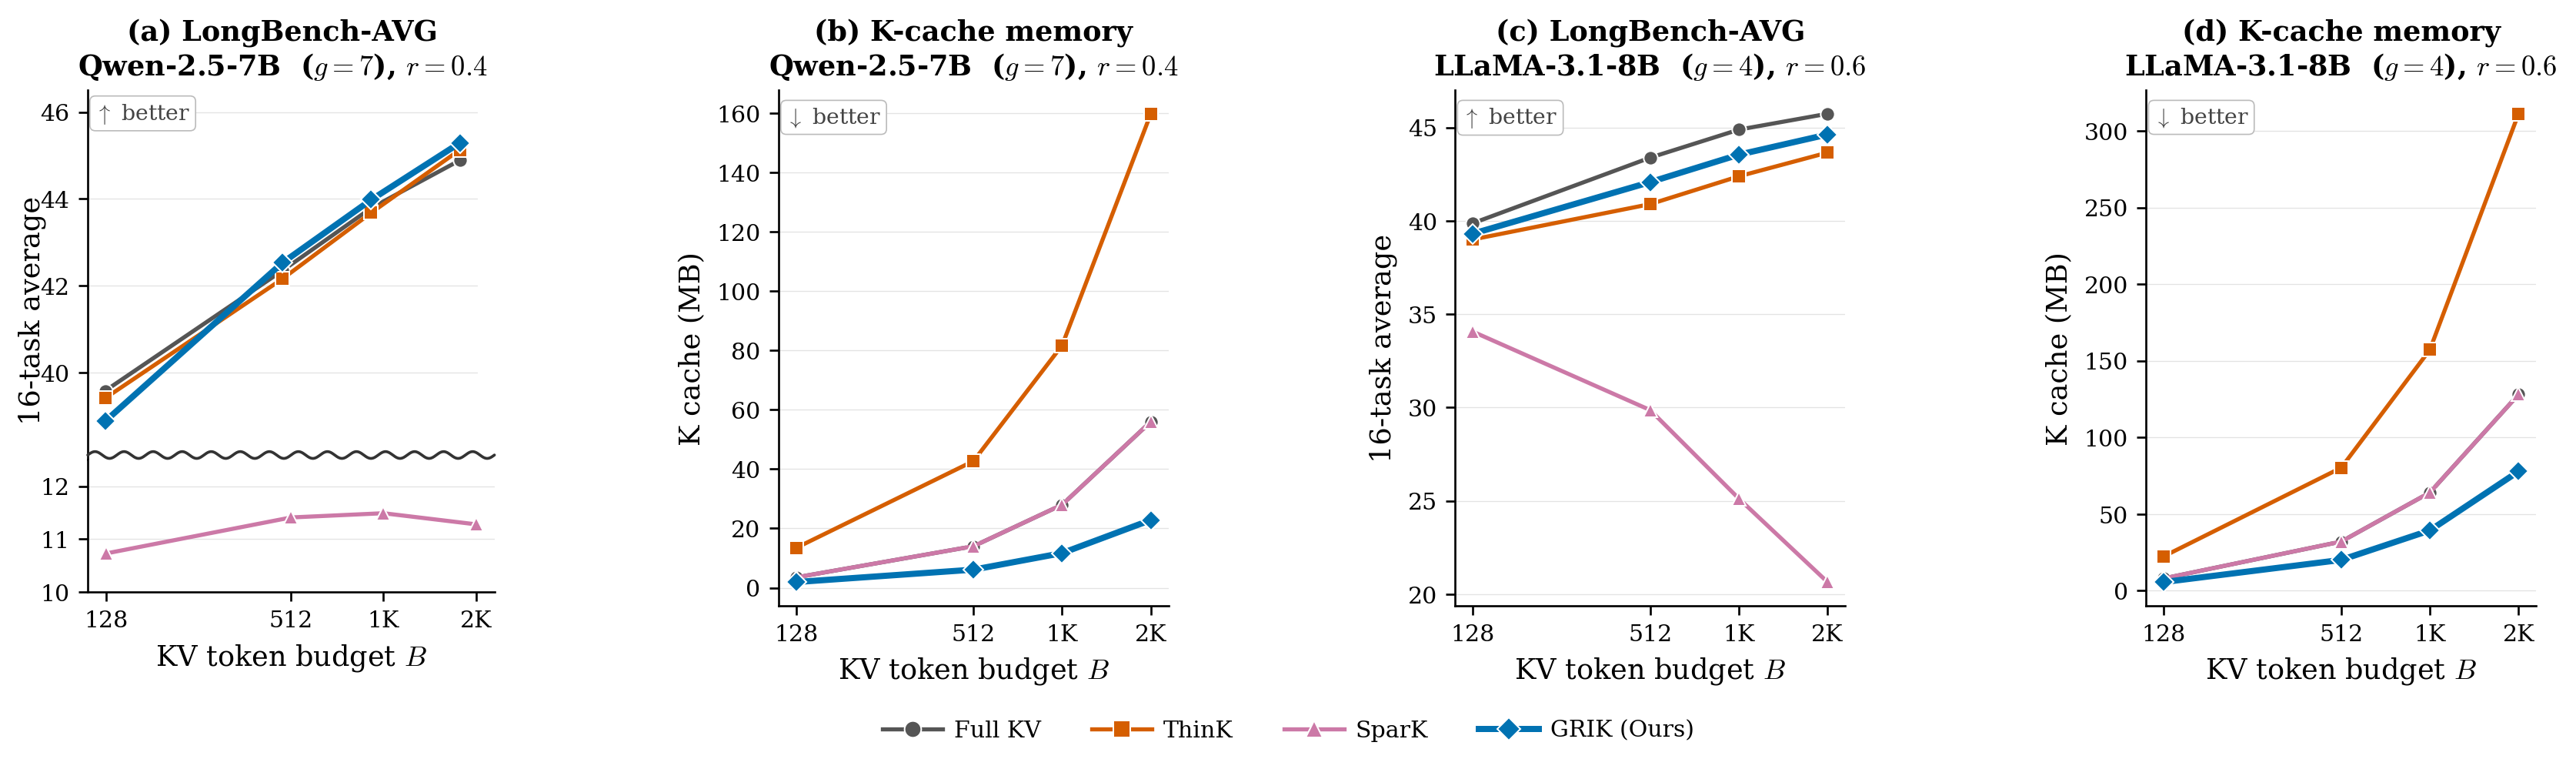
\includegraphics[width=\textwidth]{figs/scorecard_qwen_llama31.png}
\caption{\textbf{Accuracy and K-cache memory vs.\ KV budget $B$.} \textbf{(a)--(b)} Qwen-2.5-7B ($g{=}7$, $r{=}0.4$); \textbf{(c)--(d)} LLaMA-3.1-8B ($g{=}4$, $r{=}0.6$). GRIK is the only method whose accuracy tracks Full~KV while its K-cache stays below the Full~KV reference at every $B$. ThinK pays $7\times$/$4\times$ memory premiums; SparK collapses on both pairs (Appendix~\ref{app:storage-degradation}).}
\label{fig:scorecard}
\end{figure*}
% ============================================================
\section{GRIK: Grouped Relevance-Integrated Key Pruning}
\label{sec:method}
% ============================================================
 
The structural analysis in \S\ref{sec:preliminaries} reduces channel pruning under GQA to a single object: a per-KV-head mask $M_{h_{\mathrm{kv}}} \in \{0,1\}^d$ shared by all query heads in the group and applied uniformly across tokens. GRIK is the simplest training- and calibration-free instantiation of this constraint. The channel score combines three measurable signals---the output-projection influence $\alpha_h$ of each query head, the static prior $w_k$ from the K-projection row norms, and the prompt-specific dynamic signal $E_q \cdot E_k$ from attention energy---into a single per-KV-head score:
\begin{equation}
s_{h_{\mathrm{kv}}}[d'] \;=\; \underbrace{w_k[h_{\mathrm{kv}}, d']}_{\text{static prior}} \cdot \sum_{h \in \mathcal{G}_{h_{\mathrm{kv}}}} \alpha_h \cdot \underbrace{E_q[h, d'] \cdot E_k[h_{\mathrm{kv}}, d']}_{\text{dynamic signal}}.
\label{eq:score}
\end{equation}
The mask is taken as $M_{h_{\mathrm{kv}}} = \mathrm{Top}\text{-}k(s_{h_{\mathrm{kv}}}, k)$ at retention $k = \lfloor rd \rfloor$. Definitions of $\alpha_h$, $w_k$, $E_q$, $E_k$, and the rationale for each term are provided in Appendix~\ref{app:method-details}.
 
\paragraph{Iterative refinement.}
The dynamic signal depends on the attention distribution, which itself depends on the mask, so a one-shot computation from full-cache energies cannot account for the energy distribution under the pruned state. GRIK addresses this mutual dependence with an $N$-step schedule: at step $t$, attention is recomputed under the current mask, energies $E_q^{(t)}$ and $E_k^{(t)}$ are updated, and the mask contracts one step toward $\lfloor rd \rfloor$. We use $N=32$ throughout. A unit-variance correction (replacing $\sqrt{d}$ with $\sqrt{k_t}$ in the scaled dot product) is applied inside the loop to keep logit magnitudes consistent with the unpruned $\sqrt{d}$ scaling at deployment time; Appendix~\ref{app:variance} verifies that this is exactly the rescaling that preserves the logit variance assumed by the pre-trained model. Full pseudocode and the definitions of $\alpha_h$, $w_k$, $E_q$, $E_k$ are given in Appendix~\ref{app:method-details} (Algorithm~\ref{alg:grik}).
 
\paragraph{Complexity.}
GRIK's cost is concentrated in prefill and adds no decoding-time overhead. Per layer, computing $\alpha_h$, $E_q$, and $E_k$ takes $O(HTd)$, and the $N$-step refinement adds $O(N \cdot H_{\mathrm{kv}} \cdot d \log d)$ for top-$k$ selection. For $N=32$ this is negligible relative to prefill attention's $O(HT^2d)$. At decoding, the pruned K cache is stored as a dense tensor in $\mathbb{R}^{H_{\mathrm{kv}} \times T \times k}$, so existing FlashAttention-style kernels apply unmodified. We report measured memory reductions in \S\ref{sec:memory}.
 
 
 
 
 
 
% ============================================================
\section{Experiments}
\label{sec:experiments}
% ============================================================
 
Figure~\ref{fig:scorecard} previews the headline result of this section: at two complementary long-context operating points --- Qwen-2.5-7B-Instruct ($g{=}7$, $r{=}0.4$) and LLaMA-3.1-8B-Instruct ($g{=}4$, $r{=}0.6$) --- GRIK is the only channel-pruning method whose accuracy trajectory tracks Full~KV while its memory trajectory stays below the Full~KV reference at every KV token budget. The remainder of \S\ref{sec:experiments} unpacks this picture: \S\ref{sec:longbench} reports per-backbone LongBench results across the full grid; \S\ref{sec:ruler} stress-tests the methods on RULER at growing sequence lengths in the no-eviction regime; \S\ref{sec:memory} validates the K-cache curves of Figure~\ref{fig:scorecard} against the per-token storage formula and the realized cache tensors; \S\ref{sec:ablation} isolates the contribution of GRIK's score components.
 





% ============================================================





\subsection{Settings}
\label{sec:settings}


\begin{table}[t!]
\centering
\small
\setlength{\tabcolsep}{4pt}
\renewcommand{\arraystretch}{1.10}
\caption{LongBench-v1 16-task average across three GQA backbones, four KV budgets, retention ratios $r{=}\{0.4, 0.6\}$ (H2O eviction). \textbf{Bold} marks the best non-Full-KV cell per (model, budget, ratio). Rightmost column: asymptotic K-cache ratio vs.\ Full~KV (GRIK $= r$, SparK $= 1{\times}$, ThinK $= g{\cdot}r$). Per-task tables and the no-eviction column in Appendix~\ref{app:longbench-pertask}.}
\label{tab:main_avg}
\begin{tabular}{llrrrrr}
\toprule
Model & Method & $B{=}128$ & $B{=}512$ & $B{=}1024$ & $B{=}2048$ & K-cache \\
\midrule
\multirow{7}{*}{LLaMA-3-8B-Inst.}
& Full KV (reference)$^\ast$            & 35.38          & 37.23          & 38.70          & 39.59          & $1.00\times$ \\
\cmidrule(lr){2-7}
& ThinK ($r{=}0.4$)            & 35.63          & 37.39          & 39.00          & 40.05          & $1.60\times$ \\
& SparK ($r{=}0.4$)                      & 32.73          & 33.92          & 34.68          & 34.83          & $1.00\times$ \\
& \textbf{GRIK ($r{=}0.4$)}              & \textbf{35.92} & \textbf{38.63} & \textbf{40.12} & \textbf{41.30} & $\mathbf{0.40\times}$ \\
\cmidrule(lr){2-7}
& ThinK ($r{=}0.6$)            & 35.06          & 36.44          & 37.58          & 38.51          & $2.40\times$ \\
& SparK ($r{=}0.6$)                      & 27.97          & 26.62          & 24.11          & 21.92          & $1.00\times$ \\
& \textbf{GRIK ($r{=}0.6$)}              & \textbf{35.00} & \textbf{37.45} & \textbf{38.45} & \textbf{39.24} & $\mathbf{0.60\times}$ \\
\midrule
\multirow{7}{*}{LLaMA-3.1-8B-Inst.}
& Full KV (reference)                    & 39.87          & 43.38          & 44.88          & 45.73          & $1.00\times$ \\
\cmidrule(lr){2-7}
& ThinK ($r{=}0.4$)                      & 39.22          & 41.56          & 42.79          & 44.30          & $1.60\times$ \\
& SparK ($r{=}0.4$)                      & 38.22          & 39.94          & 39.94          & 38.47          & $1.00\times$ \\
& \textbf{GRIK ($r{=}0.4$)}              & \textbf{39.60} & \textbf{43.17} & \textbf{44.63} & \textbf{45.46} & $\mathbf{0.40\times}$ \\
\cmidrule(lr){2-7}
& ThinK ($r{=}0.6$)                      & 39.00          & \textbf{40.89} & \textbf{42.38} & 43.65          & $2.40\times$ \\
& SparK$^\ddagger$ ($r{=}0.6$)           & 34.06          & 29.86          & 25.12          & 20.65          & $1.00\times$ \\
& \textbf{GRIK ($r{=}0.6$)}              & \textbf{39.31} & \textbf{42.07} & \textbf{43.54} & \textbf{44.62} & $\mathbf{0.60\times}$ \\
\midrule
\multirow{7}{*}{Qwen2.5-7B-Inst.}
& Full KV (reference)                    & 39.58          & 42.35          & 43.79          & 44.89          & $1.00\times$ \\
\cmidrule(lr){2-7}
& ThinK ($r{=}0.4$)                      & \textbf{39.41} & 42.16          & 43.68          & 45.13          & $2.80\times$ \\
& SparK ($r{=}0.4$)                      & 10.73          & 11.41          & 11.49          & 11.28          & $1.00\times$ \\
& \textbf{GRIK ($r{=}0.4$)}              & 38.88          & \textbf{42.53} & \textbf{43.98} & \textbf{45.29} & $\mathbf{0.40\times}$ \\
\cmidrule(lr){2-7}
& ThinK ($r{=}0.6$)                      & \textbf{39.40} & 41.93          & \textbf{43.64} & \textbf{44.92} & $4.20\times$ \\
& SparK ($r{=}0.6$)                      & 10.55          & 10.93          & 10.98          & 10.86          & $1.00\times$ \\
& \textbf{GRIK ($r{=}0.6$)}              & 38.27          & \textbf{42.05} & 43.49          & 44.73          & $\mathbf{0.60\times}$ \\
\bottomrule
\end{tabular}
\end{table}






We evaluate GRIK on three GQA backbones --- LLaMA-3-8B-Instruct, LLaMA-3.1-8B-Instruct~\citep{llama3}, and Qwen-2.5-7B-Instruct~\citep{qwen25} --- across two long-context benchmarks: LongBench-v1~\citep{longbench} (16 tasks, six categories) and RULER~\citep{ruler} (13 synthetic subtasks at sequence lengths $\{4\text{K}, 8\text{K}, 16\text{K}, 32\text{K}\}$). The three backbones span GQA group factors $g \in \{4, 4, 7\}$ and head-dimension layouts. We compare GRIK against three channel-pruning baselines --- Full~KV (no channel pruning), ThinK~\citep{think}, and SparK~\citep{spark} --- plus the GQA-storage-matched variant ThinK-GQA-mean introduced in~\S\ref{sec:diagnosis}; all baselines use the H2O~\citep{h2o} eviction prefix at the same token budget so that quality gaps reflect channel-level effects. We sweep KV token budgets $B \in \{128, 256, 512, 1024, 2048\}$ and the no-eviction regime ($B = \infty$, channel-only) at retention ratios $r \in \{0.4, 0.6\}$ ($60\%$ and $40\%$ kept), with recent window $w = 32$. Full setup details --- per-model architectural specs, dataset/metric protocols, baseline implementations, hardware, and hyperparameters --- are deferred to Appendix~\ref{app:expsetup}.



\subsection{Long-Context Benchmark}
\label{sec:longbench}
% ============================================================






Table~\ref{tab:main_avg} reports LongBench-v1 16-task averages across three GQA backbones, two retention ratios, and four KV budgets ($24$ measurement cells); per-task tables and the no-eviction column are in Appendix~\ref{app:longbench-pertask}.
 
\paragraph{Quality.} GRIK is the strongest non-Full-KV method on $19/24$ cells, within $0.6$ points of the leader on $4$ of the remaining $5$ and within $1.13$ on the last; the five losses are all to ThinK at $B{=}128$ or on Qwen-2.5 at $r{=}0.6$. On LLaMA-3.1-8B at $r{=}0.4$, GRIK trails Full~KV by at most $0.27$ points at every budget while ThinK loses $0.65\text{--}2.09$ and SparK $1.65\text{--}7.26$. SparK collapses uniformly on Qwen-2.5 (AVG $\sim 11$ regardless of $B$): per-token recovery in a $g{=}7$ group amplifies channel-removal noise (Appendix~\ref{app:storage-degradation}). At $r{=}0.6$ SparK degrades further on every backbone (LLaMA-3.1: $34.06 \to 20.65$ across $B \in [128, 2048]$); GRIK and ThinK degrade gracefully and GRIK retains its lead.
 

 
\paragraph{Memory.} The rightmost column of Table~\ref{tab:main_avg} reports the asymptotic K-cache footprint vs.\ Full~KV: GRIK $= r$ (always below $1\times$), SparK $= 1\times$ (no reduction), ThinK $= g \cdot r$ (up to $4.20\times$ on Qwen-2.5 at $r{=}0.6$). Combined with the accuracy columns, GRIK occupies the strict (memory, quality) Pareto frontier at every operating point; Figure~\ref{fig:scorecard} reads the same conclusion off the budget axis.
 

% ============================================================
\subsection{Synthetic Long-Context Stress Test (RULER)}
\label{sec:ruler}
% ============================================================
 
LongBench averages can mask method-specific failure modes. RULER isolates exact-string retrieval at controlled context lengths and is therefore a sharper test of condition C2.
 
Table~\ref{tab:ruler-summary} reports RULER averages at $\{4\text{K}, 8\text{K}, 16\text{K}, 32\text{K}\}$ on LLaMA-3.1-8B-Instruct in the no-eviction regime ($r{=}0.7$, KV $200$K). SparK averages below $7$ at every length, with all eight needle-in-a-haystack subtasks scoring $0\%$: per-token recovery fills dropped channels with noise, destroying the precise key signature retrieval requires. GRIK averages $54$--$62$ over the same range, retaining most of Full~KV retrieval at $4$K and declining gradually with length. The dissociation makes the structural reading of \S\ref{sec:conditions} concrete: condition C2 is functionally required for retrieval-style attention. Per-task breakdowns and a detailed mechanism analysis are in Appendix~\ref{app:ruler-pertask}; the 4K--16K results were measured on an A6000 (48~GiB) and the 32K result on an RTX PRO 6000 (96~GiB) with SDPA prefill.
 
\begin{table}[t!]
\centering
\small
\setlength{\tabcolsep}{4pt}
\renewcommand{\arraystretch}{1.15}
\caption{RULER on LLaMA-3.1-8B-Instruct, $r{=}0.7$, KV budget $200$K (channel-only). $^\dagger$ Cited at the matched setting; Avg.\ recomputed over the four lengths shown.}
\label{tab:ruler-summary}
\begin{tabular}{@{}l rrrr r@{}}
\toprule
\textbf{Method} & \textbf{4K} & \textbf{8K} & \textbf{16K} & \textbf{32K} & \textbf{Avg.} \\
\midrule
\textit{Llama-3.1-8B}\,$^\dagger$  & 95.10 & 93.10 & 90.20 & 86.00 & 91.10 \\
ThinK~\citep{think}\,$^\dagger$    & 58.30 & 39.20 & 37.50 & 36.40 & 42.85 \\
SparK~\citep{spark}                &  6.17 &  3.80 &  3.32 &  2.58 &  3.97 \\
\rowcolor{gray!15}
\textbf{GRIK} (Ours)               & \textbf{61.52} & \textbf{60.00} & \textbf{56.70} & \textbf{54.24} & \textbf{58.12} \\
\bottomrule
\end{tabular}
\end{table}
 
 
% ============================================================
\subsection{Memory Efficiency}
\label{sec:memory}
% ============================================================



The accuracy results above are obtained under a strict same-token-budget comparison; the realized memory cost varies dramatically across methods. The per-layer K-cache size in 16-bit storage is
\[
\text{Bytes}_{\text{K}} = H_{*} \cdot \big[(B-w)\,k_{*} + w\,d\big] \cdot 2,
\]
where $(H_{*}, k_{*}) = (H_{kv}, d)$ for Full~KV and SparK (recovered to dense), $(H_q, k)$ for ThinK, and $(H_{kv}, k)$ for GRIK; Appendix~\ref{app:storage-invariance} gives the formal characterization, and the formula matches the materialized PyTorch tensors within $0.1\%$ (Appendix~\ref{app:memory-validation}). On LLaMA-3-8B at $r{=}0.4$ ($H_q{=}32, H_{kv}{=}8, d{=}128, k{=}51$), the three layouts yield ThinK $\approx 3.2\times$ Full~KV (per-Q-head storage scales as $g \cdot r$; Appendix~\ref{app:storage-degradation}), SparK $1.00\times$ (per-token masks preclude shape reduction; Appendix~\ref{app:storage-degradation}), and GRIK $0.60\times$ (both conditions hold). Numerical detail across $B$ and $r$ is given in Table~\ref{tab:memory-grid} (Appendix~\ref{app:memory-validation}).


% \begin{wrapfigure}{r}{0.54\textwidth}
% \centering
% \vspace{-10pt}
% 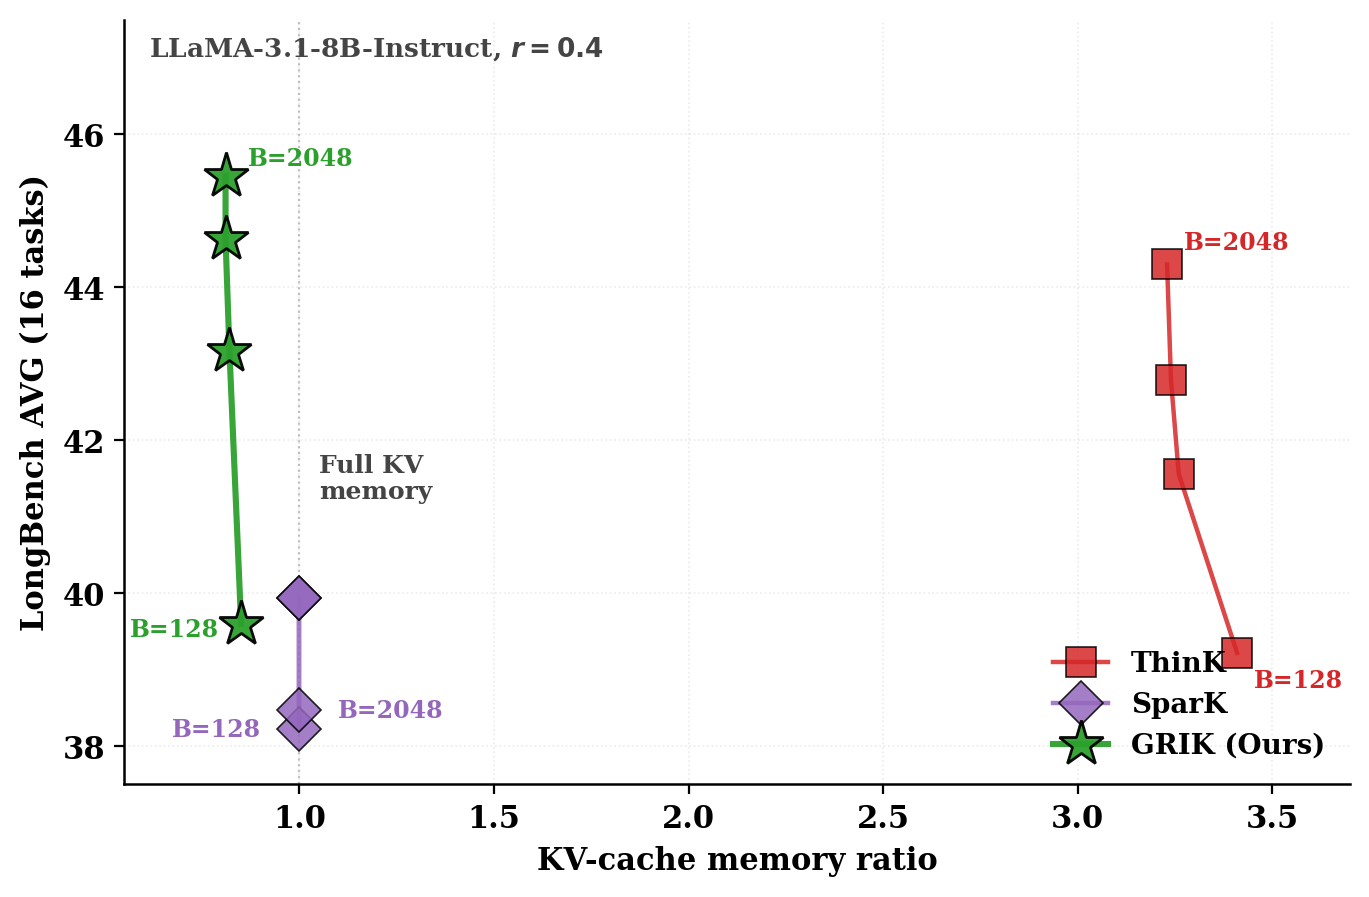
\includegraphics[width=0.52\textwidth]{figs/pareto.png}
% \caption{\textbf{Memory--accuracy Pareto frontier.} LLaMA-3.1-8B-Instruct, $r{=}0.4$. GRIK lies upper-left of ThinK and SparK at every budget $B \in \{128, 512, 1024, 2048\}$.}
% \label{fig:pareto}
% \end{wrapfigure}
% \vspace{-10pt}


\paragraph{Operational consequences.} At long context the K-cache size controls either the maximum servable sequence length (single-stream) or the maximum batch size (concurrent serving). In a $14$~GiB pool typical of an 8B-class model on a $48$~GiB GPU after weights and workspace, GRIK fits roughly $1.25\times$ as many context tokens as Full~KV, while ThinK fits roughly $0.31\times$. Channel pruning composes multiplicatively with per-element quantization (Appendix~\ref{app:composition}): combining GRIK with FP8 KV-cache halves the per-element cost without altering the layout, yielding $0.40\times$ the bf16 Full-KV baseline.
 
% \paragraph{Pareto view.} Figure~\ref{fig:pareto} compresses the LongBench-AVG scores from \S\ref{sec:longbench} together with the cache-memory ratios from this section into a single (memory, accuracy) plane. Each method traces a trajectory across KV budgets; GRIK's lies strictly upper-left of both ThinK and SparK at every budget --- less memory, equal-or-higher accuracy.
 
 

\subsection{Ablation}
\label{sec:ablation}
 
GRIK's score formula combines three ingredients beyond the structural choice of a single per-KV-head shared mask: (i) $\alpha_h$-weighted aggregation of within-group query-head channel preferences, (ii) the static $\|W_k\|$ prior~\citep{wanda}, and (iii) progressive iterative refinement. The structural choice itself is a prerequisite of the storage layout, not an algorithmic knob; this section isolates the contribution of (i)--(iii) by holding the layout fixed.
 
The natural reference with the same layout but none of (i)--(iii) is \textbf{ThinK-GQA-mean}: ThinK's per-query-head channel score, averaged uniformly within each KV group. ThinK-GQA-mean inherits GRIK's storage footprint exactly ($H_{kv}$ heads, $k$ channels), so any quality difference reflects the score form alone. Table~\ref{tab:ablation-and-memory}(a) reports this comparison on LLaMA-3-8B-Instruct across all four KV budgets and both retention ratios; panel (b) reports each method's K-cache footprint as a fraction of Full~KV (K+V combined) under the same grid.
 
\begin{table}[t!]
\centering
\footnotesize
\caption{\textbf{(a)}~Score-form ablation: GRIK vs.\ ThinK-GQA-mean (uniform within-group aggregation, no prior, no refinement) on LLaMA-3-8B, LongBench 16-task AVG. \textbf{(b)}~K-cache as a fraction of Full~KV (K+V combined).}
\label{tab:ablation-and-memory}
 
\begin{minipage}[t]{0.52\textwidth}
\centering
\textbf{(a)~Score-form contribution}\label{tab:channel-ablation}\\[2pt]
\setlength{\tabcolsep}{4pt}
\renewcommand{\arraystretch}{1.05}
\begin{tabular}{@{}lrrrr@{}}
\toprule
\textbf{Method} & $B{=}128$ & $B{=}512$ & $B{=}1024$ & $B{=}2048$ \\
\midrule
\multicolumn{5}{@{}l}{\textit{$r = 0.4$}} \\
ThinK-GQA-mean       & 35.45          & 36.96          & 38.11          & 39.48          \\
\textbf{GRIK (Ours)} & \textbf{35.92} & \textbf{38.63} & \textbf{40.12} & \textbf{41.30} \\
\rowcolor{gray!15}
$\Delta$             & $+0.47$        & $+1.67$        & $+2.01$        & $+1.82$        \\
\midrule
\multicolumn{5}{@{}l}{\textit{$r = 0.6$}} \\
ThinK-GQA-mean       & 34.91          & 36.30          & 37.40          & 38.30          \\
\textbf{GRIK (Ours)} & \textbf{35.00} & \textbf{37.45} & \textbf{38.45} & \textbf{39.24} \\
\rowcolor{gray!15}
$\Delta$             & $+0.09$        & $+1.15$        & $+1.05$        & $+0.94$        \\
\bottomrule
\end{tabular}
\end{minipage}%
\hfill
\begin{minipage}[t]{0.45\textwidth}
\centering
\textbf{(b)~K-cache vs.\ Full~KV}\label{tab:memory-grid}\\[2pt]
\setlength{\tabcolsep}{4pt}
\renewcommand{\arraystretch}{1.05}
\begin{tabular}{@{}lrrrr@{}}
\toprule
\textbf{Method} & $B{=}128$ & $B{=}512$ & $B{=}1024$ & $B{=}2048$ \\
\midrule
\multicolumn{5}{@{}l}{\textit{$r = 0.4$}} \\
ThinK         & $3.41\times$         & $3.26\times$         & $3.24\times$         & $3.23\times$         \\
SparK         & $1.00\times$         & $1.00\times$         & $1.00\times$         & $1.00\times$         \\
\textbf{GRIK} & $\mathbf{0.85\times}$ & $\mathbf{0.82\times}$ & $\mathbf{0.81\times}$ & $\mathbf{0.81\times}$ \\
\midrule
\multicolumn{5}{@{}l}{\textit{$r = 0.6$}} \\
ThinK         & $3.12\times$         & $2.90\times$         & $2.86\times$         & $2.84\times$         \\
SparK         & $1.00\times$         & $1.00\times$         & $1.00\times$         & $1.00\times$         \\
\textbf{GRIK} & $\mathbf{0.78\times}$ & $\mathbf{0.72\times}$ & $\mathbf{0.71\times}$ & $\mathbf{0.71\times}$ \\
\bottomrule
\end{tabular}
\end{minipage}
\end{table}
 
\paragraph{Score-form contribution grows with budget.} GRIK improves over ThinK-GQA-mean by $+0.09$ to $+2.01$ points across the eight cells; the gap is smallest at $B{=}128$ (where the recent window dominates and channel choice has limited room to act) and widens monotonically with $B$, reaching $+2.01$ at $B{=}1024$, $r{=}0.4$. Within GRIK's score form, internal ablations on LLaMA-3-8B at $B{=}128$, $r{=}0.4$ attribute $+0.10$ to iterative refinement alone, with the remaining $+0.37$ from $\alpha_h$-weighted aggregation and the Wanda prior together; alternative dynamic signals (e.g., qsnr, $\!-0.02$ to $\!-0.17$) underperform the chosen $Q^2 K^2$ form (Appendix~\ref{app:thinkmean-ablation}, Equation~\ref{eq:score}).
 
\paragraph{Storage axis dominates the ablation axis.} The accuracy gap between any GQA-respecting method (ThinK-GQA-mean, GRIK) and the original \emph{per-Q-head} ThinK is small ($\pm 0.5$ pt), but their storage gap is structural: ThinK-GQA-mean and GRIK are bound by Definition~\ref{def:shape} to a single dense $H_{kv} \times k$ K cache, whereas per-Q-head ThinK falls back to $H_q$-head storage --- a $4\times$ inflation at $r{=}0.4$ on LLaMA-3-8B (\S\ref{sec:memory}). The design choices that determine GRIK's identity are therefore storage-relevant first and accuracy-relevant second.
 
 
% ============================================================
\section{Conclusion}
\label{sec:conclusion}
% ============================================================
 
We argued that channel-level KV-cache compression for grouped-query attention LLMs is, in the first instance, a structural problem rather than a statistical one: GQA's shared-KV storage imposes group consistency (C1) and token consistency (C2) on any channel mask, and channel sparsity translates into actual storage reduction only when both hold. Existing methods --- ThinK (per-query-head, violates C1) and SparK (per-token, violates C2) --- forfeit GQA's storage gain by construction; the former \emph{inflates} the realized K cache by approximately $3.2\times$ and the latter leaves it unchanged. GRIK enforces both conditions by construction, aggregates query-head channel preferences via output-projection influence, scores channels by a static $\|W_k\|$ prior plus prompt-specific attention energy, and refines the mask iteratively. The resulting method is training- and calibration-free, transfers across three GQA backbones and channel-keep ratios without modification, and at $60\%$ retention reduces the K-cache footprint to $0.60\times$ Full~KV while matching or exceeding the strongest prior channel-pruning method on a majority of LongBench tasks. As a limitation, our analysis covers the K cache only; pruning the V cache faces a structurally different problem because V is consumed by the output projection downstream of attention, and we leave that case for future work.

\paragraph{Limitations.} Our analysis covers the K cache only; pruning V faces a structurally different problem because V is consumed by the output projection downstream of attention, and we leave it for future work. The asymptotic K-cache ratios reported here hold in the long-context limit; at small $B$ the recent window dominates and all methods converge toward Full~KV memory. The $32$-step iterative refinement adds a one-time prefill overhead measured at $+148\%$ at 4K and $+53\%$ at 32K (Appendix~\ref{app:prefill-latency}); large-batch serving workloads remain unbenchmarked. Finally, our evaluation covers dense GQA backbones with group factors $g \in \{4, 7\}$; other GQA configurations and emerging attention variants (e.g., MoE attention, sliding-window) are unexplored.
 
\bibliographystyle{plainnat}
\bibliography{references}
 
 
% \newpage
% \input{checklist.tex}
 
 
 
\newpage
\appendix
 
% ============================================================
\section{Notation}
\label{app:notation}
 
\begin{table}[h]
\centering
\small
\setlength{\tabcolsep}{6pt}
\renewcommand{\arraystretch}{1.15}
\caption{Notation used throughout the paper.}
\label{tab:notation}
\begin{tabular}{@{}ll@{}}
\toprule
\textbf{Symbol} & \textbf{Meaning} \\
\midrule
$L$ & Number of transformer layers \\
$H$ & Number of query heads \\
$H_{\mathrm{kv}}$ & Number of key/value heads (KV heads) \\
$g = H / H_{\mathrm{kv}}$ & Group size: query heads per KV head \\
$d$ & Head dimension \\
$d_{\mathrm{model}}$ & Model hidden size, $d_{\mathrm{model}} = H \cdot d$ \\
$T$ & Sequence length \\
$B$ & Token-eviction budget (number of retained past tokens) \\
$w$ & Recent-window size, $w \le B$ \\
$r \in (0, 1]$ & Channel retention ratio \\
$k = \lfloor r \cdot d \rfloor$ & Number of retained channels per KV head \\
$\mathcal{G}_{h_{\mathrm{kv}}}$ & Set of query heads sharing KV head $h_{\mathrm{kv}}$ \\
$M_{h_{\mathrm{kv}}} \in \{0,1\}^d$ & Channel mask for KV head $h_{\mathrm{kv}}$ \\
$W_k^{(h_{\mathrm{kv}})}$, $W_O^{(h)}$ & K-projection (per KV head), output projection (per Q head) \\
$\alpha_h$ & Output-projection influence of query head $h$ (Eq.~\ref{eq:alpha}) \\
$E_q[h, d']$, $E_k[h_{\mathrm{kv}}, d']$ & Per-channel query/key energy on the current prompt (Eq.~\ref{eq:dynamic}) \\
$s_{h_{\mathrm{kv}}}[d']$ & Channel score in KV head $h_{\mathrm{kv}}$ (Eq.~\ref{eq:score}) \\
$N$ & Number of refinement steps (we use $N{=}32$) \\
\bottomrule
\end{tabular}
\end{table}
 
 
% ============================================================
\section{Theoretical Analysis}
\label{app:theory}
% ============================================================
 
This appendix formalizes the structural claims used in the body of the paper. Section~\ref{app:storage-invariance} states the storage cost of the K cache under conditions (C1) and (C2) and proves that channel pruning is exactly storage-reducing only when both conditions hold. Section~\ref{app:storage-degradation} characterizes the storage cost when either condition is violated, recovering the $3.2\times$ inflation reported for ThinK and the $1.0\times$ ratio for SparK as direct consequences. Section~\ref{app:composition} states the multiplicative composition of (C1, C2)-conformant channel pruning with token eviction. Section~\ref{app:variance} proves that the unit-variance correction used inside the iterative refinement loop preserves the pre-trained logit distribution.
 
Throughout, we use the notation of Appendix~\ref{app:notation}: $L$ is the number of layers, $H_q$ and $H_{kv}$ are the numbers of query and KV heads, $g = H_q / H_{kv}$ is the GQA group size, $d$ is the per-head channel dimension, $T$ is the prefilled context length, $k = \lfloor rd \rfloor$ is the number of channels kept after pruning, and $b$ is the per-element byte count of the storage representation (e.g., $b = 2$ for bf16). The K cache occupies a single contiguous tensor per layer, and a deployed kernel is assumed to read from this tensor under the dense, row-major layout of \citet{trtllm}.
 
% ============================================================
\subsection{Storage Invariance under (C1, C2)}
\label{app:storage-invariance}
% ============================================================
 
\begin{theorem}[Storage Invariance]
\label{thm:storage-invariance}
Let $\{M_{h_{kv}}\}_{h_{kv} \in [H_{kv}]}$ be a channel mask family with $|M_{h_{kv}}| = k$ for all $h_{kv}$, and let the K cache be stored as a contiguous dense tensor of shape $H_{kv} \times T \times k$ per layer. If (C1) and (C2) of Definition~\ref{def:shape} hold, then the total K-cache storage is exactly
\begin{equation}
S_K^{\mathrm{(C1, C2)}} = b \cdot L \cdot H_{kv} \cdot T \cdot k.
\label{eq:storage-invariance}
\end{equation}
\end{theorem}
 
\begin{proof}
By (C2), the channel mask $M_{h_{kv}}$ is shared across all $T$ tokens, so the active channels of head $h_{kv}$ form a fixed subset of size $k$ that does not depend on the token index. The dense tensor for head $h_{kv}$ at layer $\ell$ is therefore $T \times k$ regardless of which $k$ channels are kept. By (C1), every Q-head $h \in \mathcal{G}_{h_{kv}}$ in the GQA group sees the same active channel set when reading from $M_{h_{kv}}$, so no separate per-Q-head storage is needed. Summing across $H_{kv}$ heads and $L$ layers and multiplying by $b$ bytes per element gives Equation~\ref{eq:storage-invariance}. The expression depends on $k$ but not on which $k$ channels are kept, so storage is invariant to the specific selection.
\end{proof}
 
\begin{remark}
Theorem~\ref{thm:storage-invariance} is the formal statement of the design target named in \S\ref{sec:method}: any channel mask family satisfying (C1) and (C2) achieves the same storage reduction $S_K = b L H_{kv} T \cdot k = (k/d)$ times the Full~KV baseline of $b L H_{kv} T \cdot d$, regardless of how $k$ channels are scored or selected. GRIK is therefore exactly storage-reducing by construction; quality of selection determines accuracy but not memory.
\end{remark}
 
% ============================================================
\subsection{Storage Degradation under Condition Violations}
\label{app:storage-degradation}
% ============================================================
 
\begin{proposition}[C1 Violation]
\label{prop:c1-violation}
Suppose (C1) is violated: at least one GQA group $\mathcal{G}_{h_{kv}}$ contains query heads $h, h' \in \mathcal{G}_{h_{kv}}$ with distinct masks $M_h^{\mathrm{query}} \neq M_{h'}^{\mathrm{query}}$. Then under the dense, contiguous-layout assumption of TRT-LLM and equivalent runtimes, the K cache for layer $\ell$ must materialize at least the union of per-Q-head masks within each KV group:
\begin{equation}
S_K^{\neg \mathrm{C1}} \;\geq\; b \cdot L \cdot H_{kv} \cdot T \cdot \min(g k, \, d).
\end{equation}
When the per-Q-head mask supports are pairwise disjoint, the union saturates this bound at $\min(gk, d)$; in particular, for $gk \geq d$ the storage degenerates to the dense baseline $b \cdot L \cdot H_{kv} \cdot T \cdot d$.
\end{proposition}
 
\begin{proof}
Fix a layer and a KV group $\mathcal{G}_{h_{kv}}$ of size $g$. Each $h \in \mathcal{G}_{h_{kv}}$ requires the channels $M_h^{\mathrm{query}}$ to compute its attention $\mathbf{q}_h \mathbf{K}_{h_{kv}}^\top$. Since $\mathbf{K}_{h_{kv}}$ is shared across the group, the kernel must access every channel that any $h \in \mathcal{G}_{h_{kv}}$ requests; equivalently, the materialized channel set is $U_{h_{kv}} := \bigcup_{h \in \mathcal{G}_{h_{kv}}} M_h^{\mathrm{query}}$. By the union bound for finite sets, $|U_{h_{kv}}| \leq \sum_{h \in \mathcal{G}_{h_{kv}}} |M_h^{\mathrm{query}}| \leq g k$, with equality iff the masks are pairwise disjoint; trivially $|U_{h_{kv}}| \leq d$ since the universe of channels has size $d$. The dense kernel cannot read non-contiguous channels, so the storage shape per KV head must materialize all $|U_{h_{kv}}|$ channels for every token, yielding storage $\geq b L H_{kv} T \cdot \min(gk, d)$.
\end{proof}
 
\begin{remark}[Numerical example: ThinK on LLaMA-3-8B]
For LLaMA-3-8B at $r = 0.6$ ($g = 4, d = 128, k = 77$), Proposition~\ref{prop:c1-violation} gives $\min(gk, d) = \min(308, 128) = 128$. The kernel must access all $128$ channels per token, while ThinK's per-Q-head index structure adds storage for the masks themselves. The realized memory ratio versus Full~KV at the same KV-token budget is $\sim 3.2\times$ rather than the naive $0.6\times$ implied by the per-element keep ratio (\S\ref{sec:memory}, Table~\ref{tab:design-axes-with-mem}).
\end{remark}
 
\begin{proposition}[C2 Violation]
\label{prop:c2-violation}
Suppose (C2) is violated: there exist token indices $t \neq t'$ and a KV head $h_{kv}$ with $M_{h_{kv}}(t) \neq M_{h_{kv}}(t')$. Then no contiguous dense layout of shape $H_{kv} \times T \times k'$ for any $k' < d$ can faithfully represent the masked tensor, and the deployed runtime must store the full tensor:
\begin{equation}
S_K^{\neg \mathrm{C2}} \;=\; b \cdot L \cdot H_{kv} \cdot T \cdot d.
\end{equation}
\end{proposition}
 
\begin{proof}
A contiguous dense layout of shape $H_{kv} \times T \times k'$ assigns the same set of $k'$ channel indices to every token $t \in [T]$ for a fixed head $h_{kv}$. By assumption, $M_{h_{kv}}(t) \neq M_{h_{kv}}(t')$, so the active channel positions at $t$ and $t'$ differ; any single fixed channel-index assignment of size $k' < d$ fails to capture both. Hence no representation of dense-tensor shape with last dimension less than $d$ exists; the runtime must allocate the full per-head dimension $d$. The recovery functions used by~\citet{spark} fill the dropped entries with samples from a fitted distribution, but the resulting tensor has shape $H_{kv} \times T \times d$, recovering the dense baseline storage.
\end{proof}
 
% ============================================================
\subsection{Composition with Token Eviction}
\label{app:composition}
% ============================================================
 
\begin{proposition}[Multiplicative Composition]
\label{prop:composition}
Let token eviction reduce the effective KV-token count from $T$ to $B \leq T$ (e.g., via H2O~\citep{h2o}). If the channel mask family satisfies (C1) and (C2) on the retained tokens, the resulting K cache occupies
\begin{equation}
S_K^{\mathrm{evict + (C1, C2)}} \;=\; b \cdot L \cdot H_{kv} \cdot B \cdot k,
\end{equation}
i.e., the token-eviction factor $B/T$ and the channel-pruning factor $k/d$ compose multiplicatively to a total storage of $(B/T)(k/d)$ relative to the Full~KV cache at the same context length.
\end{proposition}
 
\begin{proof}
Token eviction sets the effective token dimension of the dense tensor to $B$ rather than $T$; the storage formula in Theorem~\ref{thm:storage-invariance} applies with $T$ replaced by $B$. The two compression operations act on orthogonal axes of the dense $H_{kv} \times T \times k$ tensor (token axis vs.\ channel axis), so the storage ratio against the uncompressed dense tensor $H_{kv} \times T \times d$ factorizes as $(B/T) \cdot (k/d)$.
\end{proof}
 
\begin{remark}
In our experiments we report channel-pruning storage ratios with respect to the matched-budget Full~KV reference (i.e., the same H2O eviction prefix). The $0.60\times$ K-cache figure for GRIK at $r{=}0.4$ is therefore the channel factor $k/d = 51/128 \approx 0.40$ scaled to bf16 storage; combined with H2O eviction at $B \ll T$ in long contexts, the multiplicative effect can exceed an order-of-magnitude reduction.
\end{remark}
 
% ============================================================
\subsection{Unit-Variance Correction during Iterative Refinement}
\label{app:variance}
% ============================================================
 
\begin{proposition}[Logit Variance Preservation]
\label{prop:variance}
Let $\mathbf{q}, \mathbf{k} \in \mathbb{R}^d$ have independent zero-mean entries with $\mathrm{Var}(q_i) = \mathrm{Var}(k_i) = 1$ and $\mathbb{E}[q_i k_i] = 0$ for all $i \in [d]$. The standard scaled dot-product attention~\citep{vaswani2017} then produces a logit
\begin{equation}
\ell_d \;=\; \frac{1}{\sqrt{d}} \sum_{i=1}^{d} q_i k_i
\end{equation}
with $\mathrm{Var}(\ell_d) = 1$. If a channel mask $M \subset [d]$ with $|M| = k_t$ is applied at refinement step $t$, the corresponding masked logit $\ell_{k_t} := \frac{1}{\sqrt{k_t}} \sum_{i \in M} q_i k_i$ also satisfies $\mathrm{Var}(\ell_{k_t}) = 1$, whereas using the unpruned scaling factor would give variance $k_t / d$.
\end{proposition}
 
\begin{proof}
By independence and zero-mean, $\mathrm{Var}(q_i k_i) = \mathbb{E}[q_i^2 k_i^2] - \mathbb{E}[q_i k_i]^2 = \mathbb{E}[q_i^2] \mathbb{E}[k_i^2] - 0 = 1 \cdot 1 = 1$. The cross terms $\mathbb{E}[q_i k_i q_j k_j]$ for $i \neq j$ vanish under independence, so the sum $\sum_{i \in M} q_i k_i$ has variance $\sum_{i \in M} \mathrm{Var}(q_i k_i) = |M| = k_t$. Dividing by $\sqrt{k_t}$ yields unit variance. Using the unpruned scaling $1/\sqrt{d}$ instead gives variance $k_t / d$, which is below $1$ for $k_t < d$ and would shift the softmax temperature implicitly used by the pre-trained model.
\end{proof}
 
\begin{remark}
At deployment we restore the $\sqrt{d}$ scaling so that the inference-time logits are produced exactly as during the model's pre-training. The dual scaling --- $\sqrt{k_t}$ inside the refinement loop, $\sqrt{d}$ outside --- decouples the score-form numerical stability from the deployment-time correctness; without the inner correction, intermediate energy estimates $E_q^{(t)}$ and $E_k^{(t)}$ would be biased by a factor of $\sqrt{d/k_t}$ at step $t$, distorting the score in Equation~\ref{eq:score}.
\end{remark}
 
\begin{remark}[Independence assumption.]
The unit-variance assumption on $q$ and $k$ is the same one underlying the original $1/\sqrt{d}$ scaling of \citet{vaswani2017}. In practice query and key components of a trained transformer are not exactly independent or unit-variance, but layer normalization keeps their per-component scale within a small constant, and the empirical effect of replacing $\sqrt{d}$ by $\sqrt{k_t}$ during refinement is to keep the softmax temperature within the operating regime the pre-trained model was optimized for. The ablation in Appendix~\ref{app:thinkmean-ablation} shows this matters: ThinK-mean, which uses one-shot scoring without the unit-variance correction, underperforms GRIK on every measured cell despite identical storage.
\end{remark}
 
 
% ============================================================
\section{Method Details}
\label{app:method-details}
% ============================================================
 
This appendix provides the full definitions of the three signals that compose the channel score in Equation~\ref{eq:score} (output-projection influence $\alpha_h$, static prior $w_k$, dynamic signal $E_q \cdot E_k$), together with the iterative-refinement procedure and the unit-variance correction referenced in \S\ref{sec:method}.
 
\subsection{Output-Projection Influence}
\label{app:alpha}
 
\paragraph{Background.} Attention heads are known to contribute unequally to model output. \citet{michel2019heads} demonstrated that a substantial fraction of heads in trained transformers can be removed at test time with little degradation, and \citet{voita2019analyzing} showed that a small number of specialized heads carry functionally distinct roles. We reuse this insight not for head removal but as a criterion for weighting channel preferences within a GQA group.
 
\paragraph{Definition.} The attention output $\mathbf{a}_h \in \mathbb{R}^d$ of query head $h$ contributes $W_O^{(h)} \mathbf{a}_h \in \mathbb{R}^{d_{\mathrm{model}}}$ to the residual stream. We define the output-projection influence of head $h$ as the expected magnitude of this contribution:
\begin{equation}
\alpha_h = \mathbb{E}_{\mathbf{x} \sim \mathcal{D}} \left[ \left\| W_O^{(h)} \mathbf{a}_h(\mathbf{x}) \right\|_2 \right],
\label{eq:alpha}
\end{equation}
where $\mathcal{D}$ is the set of prefilled tokens. $\alpha_h$ quantifies the effective influence of head $h$ on the residual stream, so heads with smaller $\alpha_h$ receive correspondingly smaller weight in the group-shared mask decision (Eq.~\ref{eq:score}). Compared to a uniform average across query heads in a group, the $\alpha$-weighted aggregation lets heads with higher effective influence shape the mask more strongly; we isolate this contribution against a uniform-mean baseline (ThinK-GQA-mean) in \S\ref{sec:ablation}.
 
\subsection{Static Prior and Dynamic Signal}
\label{app:score-terms}
 
GRIK defines channel importance as the product of a weight-level static prior and a prompt-specific dynamic signal. This product structure extends the principle established in LLM compression research---that channel importance scales with the combination of weight magnitude and activation magnitude~\citep{wanda, awq}---to the GQA channel-selection setting.
 
\paragraph{Static prior.} We use the channel-wise row norm of the K-projection:
\begin{equation}
w_k[h_{\mathrm{kv}}, d'] = \left\| W_k^{(h_{\mathrm{kv}})}[:, d'] \right\|_2, \quad d' \in [d].
\label{eq:static}
\end{equation}
This quantity reflects the weight energy the trained model has allocated to each channel and serves as a prompt-agnostic base importance.
 
\paragraph{Dynamic signal.} We aggregate per-channel energy on the current prompt separately on the query and key sides:
\begin{equation}
E_q[h, d'] = \mathbb{E}_t \left[ q_{h, t, d'}^2 \right], \qquad
E_k[h_{\mathrm{kv}}, d'] = \mathbb{E}_t \left[ k_{h_{\mathrm{kv}}, t, d'}^2 \right].
\label{eq:dynamic}
\end{equation}
The product $E_q \cdot E_k$ reflects the contribution of each channel to the attention dot product on the current prompt. Related attention-based dynamic importance signals have been used for token-level KV compression~\citep{h2o, snapkv, think}; we apply the same principle along the channel axis.
 
\subsection{Iterative Refinement}
\label{app:iterative}
 
\paragraph{Mutual dependence.} The score in Equation~\ref{eq:score} depends on $E_q$ and $E_k$; these energies depend on the attention distribution; the attention distribution depends on the current mask. A one-shot selection computed from the energies of the unpruned cache cannot directly predict the energies that would be observed under a pruned state, and the resulting mask can be suboptimal.
 
\paragraph{Iterative schedule.} GRIK uses an $N$-step schedule to address this mutual dependence. Iterative pruning has long been observed to outperform one-shot pruning~\citep{han2015learning, frankle2019lottery}; we apply this principle in the training-free channel-selection setting. At each step $t \in [N]$:
\begin{enumerate}
    \item Construct the pruned K cache under the current mask $M_{h_{\mathrm{kv}}}^{(t-1)}$.
    \item Recompute attention under the pruned K to update $E_q^{(t)}$ and $E_k^{(t)}$.
    \item Compute $s_{h_{\mathrm{kv}}}^{(t)}$ from the updated energies and contract the mask one step toward the target retention $\lfloor rd \rfloor$.
\end{enumerate}
The mask reaches the target after $N$ steps; we use $N=32$ in all experiments.
 
\paragraph{Unit-variance correction.} During refinement, only $k_t < d$ channels are active at intermediate steps. Scaled dot-product attention~\citep{vaswani2017} divides by $\sqrt{d}$ under the assumption that query and key components are independent and unit-variance, yielding a dot-product variance of $d$; with only $k_t$ active channels this variance is approximately $k_t$, so we divide by $\sqrt{k_t}$ inside the refinement loop to keep logit magnitudes aligned with the training-time distribution. At deployment time we restore the $\sqrt{d}$ scaling so that the pre-trained model's behavior is preserved. This dual scaling supports numerical stability during refinement and accuracy preservation at decoding.
 
\subsection{Pseudocode}
 
The complete GRIK channel-mask computation is summarized in Algorithm~\ref{alg:grik}.
 
\begin{algorithm}[h]
\caption{GRIK channel mask computation}
\label{alg:grik}
\begin{algorithmic}[1]
\Require Prefilled $\mathbf{Q}, \mathbf{K}$; retention ratio $r$; refinement steps $N$
\Ensure Group-shared channel mask $\{M_{h_{\mathrm{kv}}}\}_{h_{\mathrm{kv}} \in [H_{\mathrm{kv}}]}$
\State Compute $\alpha_h$ for all $h \in [H]$ \Comment{output-projection influence}
\State Compute $w_k[h_{\mathrm{kv}}, :]$ for all $h_{\mathrm{kv}} \in [H_{\mathrm{kv}}]$ \Comment{K-projection row norms}
\State Initialize $M_{h_{\mathrm{kv}}}^{(0)} \gets \mathbf{1}_d$ for all $h_{\mathrm{kv}}$
\For{$t = 1, \ldots, N$}
    \State $k_t \gets$ scheduled count \Comment{decreases from $d$ to $\lfloor rd \rfloor$}
    \State Compute $E_q^{(t)}, E_k^{(t)}$ under $\{M_{h_{\mathrm{kv}}}^{(t-1)}\}$ with $\sqrt{k_t}$ scaling
    \State $s_{h_{\mathrm{kv}}}^{(t)}[d'] \gets w_k[h_{\mathrm{kv}}, d'] \cdot \sum_{h \in \mathcal{G}_{h_{\mathrm{kv}}}} \alpha_h \, E_q^{(t)}[h, d'] \, E_k^{(t)}[h_{\mathrm{kv}}, d']$
    \State $M_{h_{\mathrm{kv}}}^{(t)} \gets \textsc{TopK}(s_{h_{\mathrm{kv}}}^{(t)}, k_t)$ for all $h_{\mathrm{kv}}$
\EndFor
\State \Return $\{M_{h_{\mathrm{kv}}}^{(N)}\}$
\end{algorithmic}
\end{algorithm}
 
 
% ============================================================
\section{Experimental Setup}
\label{app:expsetup}
% ============================================================
 
This appendix gives the full setup for the experiments summarized in \S\ref{sec:settings}: per-backbone architectural specifications (\S\ref{app:expsetup-models}), benchmark protocols and metrics (\S\ref{app:expsetup-data}), baseline implementation details (\S\ref{app:expsetup-baselines}), and hardware/runtime configurations (\S\ref{app:expsetup-hw}).
 
\subsection{Base Models}
\label{app:expsetup-models}
 
We evaluate GRIK across three GQA-based instruction-tuned LLMs spanning two model families and three GQA configurations. Architectural specifications are summarized in Table~\ref{tab:backbone-specs}.
 
\begin{table}[h]
\centering
\small
\setlength{\tabcolsep}{6pt}
\renewcommand{\arraystretch}{1.10}
\caption{Backbone architectures used in our experiments. $L$ = transformer layers; $H_q$, $H_{kv}$ = query and KV heads; $g = H_q / H_{kv}$ = GQA group size; $d$ = per-head channel dimension; $d_{\text{model}}$ = hidden size; $d_{\text{ffn}}$ = feed-forward inner dimension; $V$ = vocabulary size.}
\label{tab:backbone-specs}
\begin{tabular}{@{}l c c c c c c c c c@{}}
\toprule
\textbf{Model} & $L$ & $H_q$ & $H_{kv}$ & $g$ & $d$ & $d_{\text{model}}$ & $d_{\text{ffn}}$ & $V$ & \textbf{max ctx} \\
\midrule
LLaMA-3-8B-Instruct        & 32 & 32 &  8 & 4 & 128 & 4096 & 14336 & 128256 &  8K \\
LLaMA-3.1-8B-Instruct      & 32 & 32 &  8 & 4 & 128 & 4096 & 14336 & 128256 & 128K \\
Qwen-2.5-7B-Instruct       & 28 & 28 &  4 & 7 & 128 & 3584 & 18944 & 152064 & 128K \\
\bottomrule
\end{tabular}
\end{table}
 
\paragraph{LLaMA-3-8B-Instruct.} Native context length 8K, no RoPE scaling. We use the released weights at the standard precision (bfloat16). The relatively small group factor $g=4$ makes the GQA-induced storage savings of GRIK proportionally moderate ($k/d \cdot 1/g$ of MHA storage at the same $r$), but the structural pattern is identical to the higher-$g$ models.
 
\paragraph{LLaMA-3.1-8B-Instruct.} Same architecture as LLaMA-3-8B-Instruct except for RoPE scaling: a frequency factor of 8 extends the native 8K context to 128K. We load the model with \texttt{transformers} 4.45.2 to enable the \texttt{rope\_scaling} parameter; the \texttt{unsloth/Meta-Llama-3.1-8B-Instruct} mirror is used because the gated official Meta release requires special access (the weights are bit-identical). RULER experiments require the long-context capability of this backbone.
 
\paragraph{Qwen-2.5-7B-Instruct.} 28 layers, 28 query heads, 4 KV heads, hidden size 3584. The larger group factor $g=7$ amplifies both the storage gains under (C1, C2)-conformant pruning and the failure modes for (C1)/(C2) violations. We load the model in bfloat16 on an A100 80~GB.
 
\subsection{Datasets and Metrics}
\label{app:expsetup-data}
 
We evaluate on two long-context benchmarks chosen to stress complementary axes of model capability.
 
\paragraph{LongBench-v1~\citep{longbench}.} A multi-task suite of 16 datasets aggregated to a single 16-task average score (LongBench-AVG). Tasks span six categories:
\begin{itemize}\itemsep0pt
    \item \textbf{Single-document QA}: NarrativeQA, Qasper, MultiFieldQA-en (F1).
    \item \textbf{Multi-document QA}: HotpotQA, 2WikiMQA, MuSiQue (F1).
    \item \textbf{Summarization}: GovReport, QMSum, MultiNews (ROUGE-L).
    \item \textbf{Few-shot learning}: TREC (classification accuracy), TriviaQA (F1), SAMSum (ROUGE-L).
    \item \textbf{Synthetic}: PassageCount, PassageRetrieval-en (accuracy).
    \item \textbf{Code completion}: LCC, RepoBench-P (Edit-Sim).
\end{itemize}
Inputs range from 4K to 32K tokens; metric per task follows the original LongBench specification. Per-task numbers in our paper are computed with the same scoring scripts as the official benchmark.
 
\paragraph{RULER~\citep{ruler}.} A controllable synthetic long-context benchmark spanning 13 subtasks: needle-in-a-haystack variants (\texttt{niah\_single\_1/2/3}, \texttt{niah\_multikey\_1/2/3}, \texttt{niah\_multivalue}, \texttt{niah\_multiquery}), variable tracking (\texttt{vt}), common-word extraction (\texttt{cwe}), frequent-word extraction (\texttt{fwe}), and two question-answering tasks (\texttt{qa\_1}, \texttt{qa\_2}). We evaluate at sequence lengths $\{4\text{K}, 8\text{K}, 16\text{K}, 32\text{K}\}$ with 200 prompts per (task, length) cell, in the no-eviction regime (KV token budget set to 200K so that H2O eviction never fires) at retention ratio $r{=}0.7$. RULER's needle subtasks isolate \emph{exact-string retrieval}, which is the most stringent test of the token-consistency condition (C2) of Definition~\ref{def:shape}. We use the official RULER prediction harness with one minor patch: the \texttt{evaluate.py} script's heavy \texttt{nemo} dependency is replaced by a minimal manifest reader (full patch in \S\ref{app:expsetup-hw}).
 
\subsection{Baselines}
\label{app:expsetup-baselines}
 
We compare GRIK against three channel-pruning baselines and one storage-controlled GQA variant. All baselines share the same H2O~\citep{h2o} token-eviction prefix at the same KV token budget so that quality differences reflect channel-level effects only. Method-specific implementation details follow.
 
\paragraph{Full~KV.} The native GQA cache without channel pruning, paired with H2O eviction at budget $B$. Serves as the reference against which channel-pruning methods are measured at matched memory budget. For LLaMA-3-8B at $r{=}0.4$, Full~KV scores are cited from \citet{think} Table~2 (we use the same evaluation harness, prompts, and decoding configuration); for LLaMA-3.1 and Qwen-2.5 we measure Full~KV ourselves under the same configuration as the channel-pruning methods to ensure consistency.
 
\paragraph{ThinK~\citep{think}.} The standard MHA-style channel-pruning method using per-query-head, attention-magnitude scoring at the configured retention ratio. We use the authors' public implementation at \texttt{thunlp/ThinK} (commit \texttt{4cf166a}). Because each Q-head receives its own mask, the deployed K cache cannot fold back to $H_{kv}$ heads under the dense layout assumed by attention kernels; in our memory accounting (\S\ref{sec:memory}) ThinK's K cache reverts to $H_q$-head storage at $k$ channels per head, yielding a $\sim 3.2\times$ inflation at $r{=}0.6$ on LLaMA-3-8B. For LLaMA-3-8B we cite ThinK numbers from~\citet{think} Table~2 directly; for LLaMA-3.1 and Qwen-2.5 we run ThinK with the released code on the same hardware as the GRIK runs.
 
\paragraph{ThinK-GQA-mean.} A storage-controlled variant of ThinK introduced in \S\ref{sec:diagnosis}: the per-query-head ThinK score is averaged uniformly within each KV group, producing a single shared mask per KV head. This variant matches GRIK's storage footprint exactly ($H_{kv}$ heads, $k$ channels) and isolates the contribution of GRIK's $\alpha_h$-weighted aggregation, static prior, and iterative refinement from the underlying storage layout. Used only for the score-form ablation (Appendix~\ref{app:thinkmean-ablation}); not part of the main result table.
 
\paragraph{SparK~\citep{spark}.} Query-aware unstructured channel sparsity. Each token receives an independent per-channel mask; pruned entries are not packed into a reduced tensor but reconstructed in place by drawing from a per-channel distribution at the recovered position. We use the released implementation with the default \texttt{normal} recovery mode (recovery distribution: $\mathcal{N}(\mu_c, \sigma_c^2)$ where $\mu_c, \sigma_c$ are estimated per channel from the unmasked statistics). Because masks vary across tokens, condition (C2) is violated; the recovered cache has shape $H_{kv} \times T \times d$, identical to Full~KV's storage footprint (Proposition~\ref{prop:c2-violation}).
 
\paragraph{GRIK (Ours).} The method described in \S\ref{sec:method} with default hyperparameters: 32 refinement steps, $\alpha_h$-weighted aggregation, Wanda-style $\|W_k\|$ static prior~\citep{wanda}, and the unit-variance correction (Proposition~\ref{prop:variance}). The retention ratio $r$ is the only knob the user sets; the schedule for $k_t$ at intermediate refinement steps follows a linear schedule from $d$ to $\lfloor rd \rfloor$.
 
\paragraph{Common settings.} All methods use the same H2O~\citep{h2o} eviction prefix with attention-score accumulation, identical recent window $w = 32$, and identical greedy decoding (temperature 0). Channel-retention ratios swept: $r \in \{0.4, 0.6\}$. KV token budgets swept: $B \in \{128, 256, 512, 1024, 2048\}$ plus the no-eviction regime ($B = \infty$, i.e., \texttt{kv\_size} $= 200{,}000$). Recent window covers the most recent $w$ tokens that are stored at the original (unpruned) channel dimension $d$; this matches the protocol used by~\citet{think} and the H2O baseline.
 
\subsection{Hardware and Runtime}
\label{app:expsetup-hw}
 
\paragraph{Hardware.} LLaMA-3 experiments run on a single NVIDIA RTX A6000 (48~GB) box. LLaMA-3.1 LongBench experiments run on a DGX H100 cluster (single GPU per run). Qwen-2.5 experiments run on a single A100 80~GB. RULER 4K--16K runs on the A6000 box; the 32K RULER cell runs on an RTX PRO 6000 (96~GB) because peak prefill memory at 32K exceeds the A6000 envelope. The TRT-LLM KV-pool validation runs on a Hopper-class GPU using the official TensorRT-LLM 1.0.0 docker image.
 
\paragraph{Runtime configuration.} \texttt{transformers} 4.40 for LLaMA-3 and Qwen-2.5; \texttt{transformers} 4.45.2 for LLaMA-3.1 (required for \texttt{rope\_scaling}). All forward passes use eager attention (the GRIK and ThinK monkey-patches operate on the eager path); for prefill at $\geq 8$K tokens we additionally enable \texttt{prefill\_sdpa=1} which routes the prefill output projection through SDPA flash-attention while keeping cache writes on the eager path (RULER setup; see \texttt{docs/experiments/main\_table/llama3.1-8b-instruct/ruler/RUNNING.md} in the released code).
 
\paragraph{RULER patch.} The official RULER \texttt{evaluate.py} imports \texttt{nemo.collections.asr.parts.utils.manifest\_utils}, which pulls in the entire NeMo dependency tree (incompatible with our environment). We replace the import with a one-line manifest reader/writer using the standard \texttt{json} module; the patched function preserves bit-equivalent behavior on RULER's manifest format. The patch is included in our released code.
 
\paragraph{Reproducibility.} The evaluation harness, prompts, and decoding configuration are shared across all methods within a given backbone. Seeds are fixed at the dataset-loader level (LongBench/RULER both ship with deterministic prompt orderings). With the released code and the runtime configuration above, all numbers in this paper reproduce within the floating-point determinism of the underlying CUDA kernels (typically $\leq 0.05$ on a 16-task LongBench AVG).
 
 
% ============================================================
\section{Memory Validation and Detailed Memory Grid}
\label{app:memory-validation}
% ============================================================
 
\subsection{Formula vs.\ Realized Cache}
 
We validate the per-layer formula in \S\ref{sec:memory} against the actual cache tensors materialized during a forward pass on LLaMA-3.1-8B-Instruct (fp16, $H_{kv}{=}8$, $d{=}128$, $L{=}32$). Memory is summed over all $L$ layers. The eviction prefix is set so that all configurations are post-eviction (a single sequence of length $4096$ at $B{=}128$ and the noted budget), and we sum bytes over the K cache only.
 
\begin{table}[h]
\centering
\small
\setlength{\tabcolsep}{6pt}
\renewcommand{\arraystretch}{1.15}
\caption{K-cache memory measured by realized tensor shapes versus the closed-form formula in \S\ref{sec:memory}. Discrepancies are below 0.1\%.}
\label{tab:memory-validation}
\begin{tabular}{@{}llrrrc@{}}
\toprule
\textbf{Method} & \textbf{ratio} & \textbf{$B$} & \textbf{Realized (MiB)} & \textbf{Formula (MiB)} & \textbf{rel.\ error} \\
\midrule
Full KV  & ---  &   128 &  16.13 &  16.13 & $<0.01\%$ \\
Full KV  & ---  &  1024 & 127.55 & 127.55 & $<0.01\%$ \\
ThinK    & 0.4  &   128 &  54.56 &  54.59 & $0.06\%$ \\
ThinK    & 0.4  &  1024 & 413.31 & 413.27 & $0.01\%$ \\
SparK    & 0.4  &   128 &  16.13 &  16.13 & $<0.01\%$ \\
GRIK     & 0.4  &   128 &  13.64 &  13.66 & $0.13\%$ \\
GRIK     & 0.4  &  1024 & 103.33 & 103.35 & $0.02\%$ \\
GRIK     & 0.6  &   128 &   9.95 &   9.97 & $0.20\%$ \\
\bottomrule
\end{tabular}
\end{table}
 
% ============================================================
\section{Prefill Latency Measurement}
\label{app:prefill-latency}
% ============================================================
 
We measure end-to-end prefill wall-clock time on LLaMA-3-8B-Instruct at $r{=}0.4$ ($d_{\text{keep}}{=}77$), batch~$1$, bf16, on an NVIDIA GB10 GPU, across context lengths $\{4\text{K}, 8\text{K}, 16\text{K}, 32\text{K}\}$. Three configurations are compared: Full~KV prefill (SDPA backend, baseline), GRIK with $N{=}1$ refinement step (one-shot scoring), and GRIK with the default $N{=}32$. Each cell is the mean over $3$ runs after $1$ warmup, with standard deviations below $1\%$ of the mean across all measurements. End-to-end (E2E) throughput in the rightmost column is the relative tokens/sec at $16$ generated tokens, including both prefill and decoding.
 
\begin{table}[!ht]
\centering
\small
\setlength{\tabcolsep}{6pt}
\renewcommand{\arraystretch}{1.15}
\caption{Prefill wall-clock latency on LLaMA-3-8B-Instruct, $r{=}0.4$, NVIDIA GB10, bf16, batch~$1$. Overheads are relative to Full~KV prefill at the same context length. E2E column: throughput at $16$ generated tokens vs.\ Full~KV.}
\label{tab:prefill-latency}
\begin{tabular}{@{}lrrrrrr@{}}
\toprule
 & \multicolumn{2}{c}{Full~KV} & \multicolumn{2}{c}{GRIK $N{=}1$} & \multicolumn{2}{c}{GRIK $N{=}32$} \\
\cmidrule(lr){2-3}\cmidrule(lr){4-5}\cmidrule(lr){6-7}
\textbf{Context} & prefill (s) & E2E (rel.) & prefill (s) & overhead & prefill (s) & overhead \\
\midrule
4K  &  1.20 & $1.00\times$ & 1.37 & $+14.0\%$ &  2.97 & $+147.7\%$ \\
8K  &  2.46 & $1.00\times$ & 2.76 & $+11.9\%$ &  5.12 & $+108.1\%$ \\
16K &  5.19 & $1.00\times$ & 5.72 & $+10.1\%$ &  8.98 & $+73.0\%$  \\
32K & 12.05 & $1.00\times$ & 13.03 & $+8.2\%$ & 18.45 & $+53.1\%$  \\
\bottomrule
\multicolumn{7}{@{}l}{\footnotesize E2E (rel.) at 16 generated tokens: GRIK $N{=}1$ achieves $0.96$--$0.98\times$; GRIK $N{=}32$ achieves $0.62$--$0.74\times$ Full~KV.}
\end{tabular}
\end{table}
 
\paragraph{Two patterns are visible.} (i) The $N{=}32$ relative overhead falls monotonically with context length, from $+147.7\%$ at 4K to $+53.1\%$ at 32K. This is expected: Full~KV prefill is dominated by attention's $\mathcal{O}(T^2)$ scaling, while GRIK's iterative refinement loop is per-prompt and scales as $\mathcal{O}(N \cdot H_{\mathrm{kv}} \cdot d \log d)$, independent of context length $T$. The refinement cost asymptotically becomes a vanishing fraction of total prefill. (ii) One-shot ($N{=}1$) carries a uniform $\sim\!10\%$ overhead, consistent with the analytical decomposition: a single forward pass of attention statistics plus mask construction. The remaining gap between $N{=}1$ and $N{=}32$ is the $31$ additional refinement steps, costing approximately $175$~ms per step at $32$K on this hardware.
 
\paragraph{End-to-end and deployment trade-off.} At $16$ generated tokens (rightmost column), GRIK $N{=}32$ runs at $0.62$--$0.74\times$ Full~KV throughput across the context range. For deployment scenarios with long generations, the one-time prefill overhead amortizes; for short-generation serving, the latency--memory trade-off depends on whether the deployment is bound by latency or by KV-cache memory pressure. Two implementation notes affect interpretation. First, Full~KV uses the SDPA attention backend while GRIK uses the eager backend, because score computation requires intermediate $Q^2/K^2$ tensors not exposed by SDPA; a fused score-extraction kernel matching SDPA performance would close part of the $N{=}1$ gap. Second, refinement steps in our implementation are not yet batched across layers; per-layer batching would further reduce the $N{=}32$ overhead.
 
% ============================================================
\section{LongBench Detailed Results}
\label{app:longbench-pertask}
% ============================================================
 
This appendix reports per-task LongBench-v1 scores that complement the summary in Table~\ref{tab:main_avg}, grouped by backbone.
 
\subsection{LLaMA-3-8B-Instruct}
 
Table~\ref{tab:longbench-llama3} reports per-task scores at both $r{=}0.4$ and $r{=}0.6$. Full~KV at $r{=}0.4$ values are taken from \citet{think} Table~2 (LLaMA-3-8B-Instruct, H2O baseline at matched KV size). The 8h GQA-aggregated ThinK variant (ThinK-mean) is reported separately in Appendix~\ref{app:thinkmean-ablation} as a score-form ablation.
 
 
\begin{table*}[!ht]
\centering
\footnotesize
\setlength{\tabcolsep}{2pt}
\renewcommand{\arraystretch}{1.05}
\vspace{-0.5em}
\caption{Per-task LongBench on LLaMA-3-8B-Instruct, $w{=}32$, both retention ratios. \textbf{Bold}: best per-block Avg among ThinK / SparK / GRIK; ``--'': not available. Full~KV and ThinK rows at $r{=}0.4$, $B \in \{128, 512, 1024, 2048\}$, and ThinK rows at $r{=}0.6$, $B \in \{512, 1024, 2048\}$, cited from \citet{think} Table~2.}
\label{tab:longbench-llama3}
\resizebox{\linewidth}{!}{%
\begin{tabular}{@{}l *{17}{>{\centering\arraybackslash}p{2.3em}}@{}}
\toprule
 & \multicolumn{3}{c}{\textbf{Single-Doc QA}} & \multicolumn{3}{c}{\textbf{Multi-Doc QA}} & \multicolumn{3}{c}{\textbf{Summarization}} & \multicolumn{3}{c}{\textbf{Few-shot}} & \multicolumn{2}{c}{\textbf{Synth.}} & \multicolumn{2}{c}{\textbf{Code}} & \\
\cmidrule(lr){2-4} \cmidrule(lr){5-7} \cmidrule(lr){8-10} \cmidrule(lr){11-13} \cmidrule(lr){14-15} \cmidrule(lr){16-17}
\raisebox{1.6em}[0pt][0pt]{\textbf{Method}}
 & \rotatebox{60}{NrtvQA} & \rotatebox{60}{Qasper} & \rotatebox{60}{MF-en}
 & \rotatebox{60}{HotpotQA} & \rotatebox{60}{2WikiMQA} & \rotatebox{60}{Musique}
 & \rotatebox{60}{GovReport} & \rotatebox{60}{QMSum} & \rotatebox{60}{MultiNews}
 & \rotatebox{60}{TREC} & \rotatebox{60}{TriviaQA} & \rotatebox{60}{SAMSum}
 & \rotatebox{60}{PCount} & \rotatebox{60}{PRe}
 & \rotatebox{60}{Lcc} & \rotatebox{60}{RB-P}
 & \rotatebox{60}{Avg.} \\
\midrule
\multicolumn{18}{c}{\cellcolor{gray!15}\textit{\textbf{Channel retention $r=0.4$ (60\% kept)}}} \\
\midrule
\multicolumn{18}{c}{\textit{$B{=}128$}} \\
\midrule
Full KV & 22.12 & 13.20 & 31.61 & 37.79 & 32.71 & 18.45 & 20.32 & 22.02 & 21.10 & 38.50 & 87.75 & 39.14 &  5.83 & 69.50 & 55.06 & 50.97 & 35.38 \\
ThinK~\citep{think} & 22.85 & 14.55 & 29.49 & 38.63 & 30.84 & 18.90 & 20.12 & 21.96 & 20.68 & 38.50 & 86.38 & 38.40 &  5.50 & 69.17 & 57.93 & 56.12 & 35.63 \\
SparK~\citep{spark} & 20.30 &  8.74 & 23.46 & 31.51 & 28.13 & 14.42 & 19.18 & 21.23 & 20.20 & 40.50 & 89.55 & 37.13 &  6.03 & 66.48 & 50.82 & 46.02 & 32.73 \\
\textbf{GRIK} (Ours) & 21.64 & 12.31 & 31.87 & 40.69 & 31.24 & 19.31 & 19.40 & 21.75 & 19.79 & 40.50 & 89.78 & 38.98 &  5.55 & 69.50 & 57.75 & 54.72 & \textbf{35.92} \\
\midrule
\multicolumn{18}{c}{\textit{$B{=}512$}} \\
\midrule
Full KV & 23.52 & 17.93 & 34.68 & 42.11 & 33.52 & 19.92 & 22.11 & 22.56 & 23.82 & 41.00 & 90.46 & 40.20 &  5.87 & 69.50 & 56.71 & 51.69 & 37.23 \\
ThinK~\citep{think} & 23.76 & 17.80 & 33.80 & 40.39 & 30.70 & 19.09 & 21.82 & 22.51 & 23.78 & 41.00 & 90.16 & 40.67 &  5.15 & 69.25 & 60.77 & 57.58 & 37.39 \\
SparK~\citep{spark} & 21.79 & 10.21 & 27.28 & 29.81 & 26.59 & 14.98 & 21.09 & 22.79 & 23.08 & 53.50 & 90.80 & 37.78 &  6.04 & 65.26 & 47.45 & 44.19 & 33.92 \\
\textbf{GRIK} (Ours) & 23.50 & 18.76 & 37.54 & 42.49 & 29.59 & 20.42 & 21.94 & 22.57 & 23.50 & 52.50 & 90.36 & 39.76 &  5.32 & 69.33 & 61.82 & 58.76 & \textbf{38.63} \\
\midrule
\multicolumn{18}{c}{\textit{$B{=}1024$}} \\
\midrule
Full KV & 25.62 & 22.16 & 36.81 & 41.01 & 33.53 & 19.41 & 23.28 & 22.65 & 25.41 & 46.50 & 90.82 & 41.78 &  5.79 & 69.25 & 59.69 & 55.50 & 38.70 \\
ThinK~\citep{think} & 25.52 & 21.93 & 37.17 & 41.56 & 31.22 & 20.17 & 22.89 & 22.95 & 25.21 & 47.00 & 90.74 & 41.34 &  5.57 & 69.50 & 62.58 & 58.67 & 39.00 \\
SparK~\citep{spark} & 22.43 & 14.20 & 28.20 & 30.63 & 25.38 & 16.01 & 21.40 & 23.23 & 24.74 & 62.00 & 89.63 & 38.86 &  5.01 & 64.32 & 45.53 & 43.24 & 34.68 \\
\textbf{GRIK} (Ours) & 24.77 & 22.93 & 38.49 & 42.82 & 31.95 & 20.40 & 23.32 & 22.61 & 25.33 & 63.00 & 90.36 & 40.11 &  5.30 & 68.96 & 61.83 & 59.80 & \textbf{40.12} \\
\midrule
\multicolumn{18}{c}{\textit{$B{=}2048$}} \\
\midrule
Full KV & 25.56 & 26.85 & 39.54 & 44.30 & 32.92 & 21.09 & 24.68 & 23.01 & 26.16 & 53.00 & 90.65 & 41.84 &  4.91 & 69.25 & 58.43 & 51.31 & 39.59 \\
ThinK~\citep{think} & 25.56 & 26.31 & 39.20 & 42.96 & 31.81 & 20.53 & 24.23 & 23.35 & 25.90 & 53.50 & 90.56 & 41.03 &  5.52 & 69.25 & 62.10 & 59.00 & 40.05 \\
SparK~\citep{spark} & 24.51 & 13.87 & 27.46 & 30.45 & 24.95 & 11.90 & 21.50 & 23.15 & 25.36 & 68.00 & 89.44 & 38.14 &  4.13 & 65.46 & 46.57 & 42.40 & 34.83 \\
\textbf{GRIK} (Ours) & 25.46 & 28.05 & 38.80 & 43.06 & 31.18 & 21.06 & 25.14 & 23.03 & 26.26 & 71.00 & 90.42 & 40.97 &  4.73 & 69.17 & 62.66 & 59.87 & \textbf{41.30} \\
\midrule
\multicolumn{18}{c}{\textit{No-evict (channel-only ceiling)}} \\
\midrule
Full KV & 25.56 & 32.27 & 39.71 & 43.56 & 35.09 & 21.18 & 28.71 & 23.26 & 26.64 & 73.50 & 90.48 & 42.33 &  4.80 & 69.25 & 59.29 & 54.05 & 41.86 \\
ThinK~\citep{think} & 25.30 & 32.63 & 39.68 & 44.11 & 34.13 & 21.10 & 28.68 & 22.97 & 26.31 & 74.00 & 90.58 & 41.60 &  5.39 & 69.50 & 61.69 & 58.25 & \textbf{42.25} \\
SparK~\citep{spark} & 21.65 & 13.48 & 26.01 & 27.96 & 22.15 & 11.40 & 19.84 & 22.44 & 25.40 & 70.50 & 89.74 & 38.55 &  5.16 & 66.00 & 44.01 & 40.06 & 34.02 \\
\textbf{GRIK} (Ours) & 25.16 & 32.44 & 39.19 & 43.93 & 34.09 & 21.20 & 28.78 & 23.23 & 26.44 & 73.50 & 90.37 & 41.19 &  4.66 & 68.43 & 61.94 & 58.89 & 42.09 \\
\midrule
\multicolumn{18}{c}{\cellcolor{gray!15}\textit{\textbf{Channel retention $r=0.6$ (40\% kept --- aggressive pruning)}}} \\
\midrule
\multicolumn{18}{c}{\textit{$B{=}128$}} \\
\midrule
Full KV & 22.12 & 13.20 & 31.61 & 37.79 & 32.71 & 18.45 & 20.32 & 22.02 & 21.10 & 38.50 & 87.75 & 39.14 &  5.83 & 69.50 & 55.06 & 50.97 & 35.38 \\
ThinK~\citep{think} & 22.93 & 11.13 & 30.43 & 38.46 & 30.18 & 17.19 & 19.45 & 22.01 & 19.86 & 39.00 & 86.73 & 37.80 &  5.47 & 69.00 & 56.06 & 55.30 & \textbf{35.06} \\
SparK~\citep{spark} & 17.34 &  5.58 & 17.76 & 18.71 & 16.07 &  9.00 & 17.37 & 21.43 & 18.53 & 41.00 & 86.36 & 35.16 &  5.83 & 57.43 & 40.95 & 38.95 & 27.97 \\
\textbf{GRIK} (Ours) & 21.79 & 11.74 & 31.04 & 39.55 & 28.83 & 19.28 & 18.48 & 21.72 & 18.88 & 39.00 & 86.92 & 37.90 &  5.60 & 69.50 & 55.09 & 54.65 & 35.00 \\
\midrule
\multicolumn{18}{c}{\textit{$B{=}512$}} \\
\midrule
Full KV & 23.52 & 17.93 & 34.68 & 42.11 & 33.52 & 19.92 & 22.11 & 22.56 & 23.82 & 41.00 & 90.46 & 40.20 &  5.87 & 69.50 & 56.71 & 51.69 & 37.23 \\
ThinK~\citep{think} & 23.40 & 14.83 & 32.62 & 38.47 & 30.97 & 19.81 & 20.80 & 22.04 & 21.60 & 40.00 & 88.79 & 38.90 &  5.36 & 69.50 & 58.28 & 57.65 & 36.44 \\
SparK~\citep{spark} & 16.33 &  6.36 & 16.36 & 16.17 & 15.69 &  6.98 & 14.76 & 20.06 & 16.72 & 51.00 & 84.77 & 31.77 &  5.22 & 52.39 & 36.14 & 35.17 & 26.62 \\
\textbf{GRIK} (Ours) & 23.21 & 15.30 & 37.30 & 41.09 & 33.80 & 20.84 & 20.65 & 21.89 & 21.58 & 47.50 & 88.55 & 37.18 &  5.84 & 69.17 & 58.24 & 57.13 & \textbf{37.45} \\
\midrule
\multicolumn{18}{c}{\textit{$B{=}1024$}} \\
\midrule
Full KV & 25.62 & 22.16 & 36.81 & 41.01 & 33.53 & 19.41 & 23.28 & 22.65 & 25.41 & 46.50 & 90.82 & 41.78 &  5.79 & 69.25 & 59.69 & 55.50 & 38.70 \\
ThinK~\citep{think} & 24.06 & 17.80 & 37.85 & 38.63 & 29.98 & 19.40 & 21.41 & 22.32 & 23.42 & 44.50 & 90.16 & 39.43 &  5.84 & 69.50 & 58.31 & 58.73 & 37.58 \\
SparK~\citep{spark} & 13.98 &  6.59 & 12.90 & 13.13 & 10.65 &  4.77 & 12.66 & 18.61 & 14.65 & 52.75 & 77.86 & 29.06 &  4.56 & 47.98 & 33.76 & 31.83 & 24.11 \\
\textbf{GRIK} (Ours) & 25.07 & 18.73 & 39.29 & 40.43 & 32.45 & 20.08 & 20.88 & 22.57 & 22.92 & 54.50 & 88.77 & 37.63 &  5.09 & 69.00 & 59.05 & 58.69 & \textbf{38.45} \\
\midrule
\multicolumn{18}{c}{\textit{$B{=}2048$}} \\
\midrule
Full KV & 25.56 & 26.85 & 39.54 & 44.30 & 32.92 & 21.09 & 24.68 & 23.01 & 26.16 & 53.00 & 90.65 & 41.84 &  4.91 & 69.25 & 58.43 & 51.31 & 39.59 \\
ThinK~\citep{think} & 24.37 & 22.14 & 37.77 & 40.13 & 29.50 & 20.26 & 22.09 & 22.76 & 24.78 & 49.50 & 90.16 & 39.69 &  5.56 & 69.50 & 59.24 & 58.78 & 38.51 \\
SparK~\citep{spark} & 11.46 &  6.15 & 12.89 & 12.31 &  9.25 &  4.40 & 11.70 & 16.19 & 13.25 & 50.00 & 71.76 & 24.59 &  4.54 & 41.21 & 30.83 & 30.21 & 21.92 \\
\textbf{GRIK} (Ours) & 24.52 & 21.82 & 39.71 & 40.59 & 30.41 & 19.29 & 22.12 & 23.11 & 23.90 & 62.50 & 89.69 & 37.93 &  5.81 & 68.29 & 58.87 & 59.26 & \textbf{39.24} \\
\midrule
\multicolumn{18}{c}{\textit{No-evict (channel-only ceiling)}} \\
\midrule
Full KV & 25.56 & 32.27 & 39.71 & 43.56 & 35.09 & 21.18 & 28.71 & 23.26 & 26.64 & 73.50 & 90.48 & 42.33 &  4.80 & 69.25 & 59.29 & 54.05 & 41.86 \\
ThinK~\citep{think} & 24.39 & 31.20 & 41.42 & 42.39 & 32.08 & 20.80 & 25.93 & 23.14 & 25.45 & 74.00 & 90.43 & 39.06 &  5.77 & 68.62 & 59.51 & 59.51 & \textbf{41.48} \\
SparK~\citep{spark} &  6.81 &  6.14 & 10.57 &  8.00 &  6.47 &  3.70 & 11.46 & 14.68 & 13.45 & 50.50 & 58.04 & 18.92 &  4.40 & 43.97 & 30.87 & 27.50 & 19.72 \\
\textbf{GRIK} (Ours) & 24.17 & 30.43 & 41.64 & 43.29 & 33.24 & 21.05 & 24.36 & 23.28 & 24.48 & 73.00 & 88.86 & 37.57 &  5.78 & 68.29 & 58.56 & 59.07 & 41.07 \\
\bottomrule
\end{tabular}%
}
\end{table*}
 
 
\subsection{LLaMA-3.1-8B-Instruct}
 
Table~\ref{tab:longbench-llama31-ext} reports per-task scores at both retention ratios, all five KV budgets, and the no-eviction (channel-only) ceiling. All entries are our measurements; the $r{=}0.4$ sub-block matches the operating point used for the diagnostic in \S\ref{sec:diagnosis} (Table~\ref{tab:design-and-diagnosis}b) and the trajectory view in Figure~\ref{fig:scorecard}. The per-task pattern aligns with the 16-task aggregate in Table~\ref{tab:main_avg}: GRIK matches or exceeds ThinK and SparK on the majority of tasks at every budget, and the gap between GRIK and Full~KV stays below $0.27$ points at every budget at $r{=}0.4$. The largest per-task differentiation appears in retrieval-style subtasks (NarrativeQA, Qasper, HotpotQA, PassageRetrieval), consistent with the C2 dissociation tested more directly on RULER (\S\ref{sec:ruler}). At $r{=}0.6$, SparK's degradation is monotone in $B$ and concentrates on the same retrieval-heavy tasks; ThinK and GRIK degrade gracefully across all categories.
 
\begin{table*}[!ht]
\centering
\footnotesize
\setlength{\tabcolsep}{2pt}
\renewcommand{\arraystretch}{1.05}
\vspace{-0.5em}
\caption{Per-task LongBench on LLaMA-3.1-8B-Instruct, $w{=}32$, both retention ratios. \textbf{Bold}: best per-block Avg; ``--'': not available.}
\label{tab:longbench-llama31-ext}
\resizebox{\linewidth}{!}{%
\begin{tabular}{@{}l *{17}{>{\centering\arraybackslash}p{2.3em}}@{}}
\toprule
 & \multicolumn{3}{c}{\textbf{Single-Doc QA}} & \multicolumn{3}{c}{\textbf{Multi-Doc QA}} & \multicolumn{3}{c}{\textbf{Summarization}} & \multicolumn{3}{c}{\textbf{Few-shot}} & \multicolumn{2}{c}{\textbf{Synth.}} & \multicolumn{2}{c}{\textbf{Code}} & \\
\cmidrule(lr){2-4} \cmidrule(lr){5-7} \cmidrule(lr){8-10} \cmidrule(lr){11-13} \cmidrule(lr){14-15} \cmidrule(lr){16-17}
\raisebox{1.6em}[0pt][0pt]{\textbf{Method}}
 & \rotatebox{60}{NrtvQA} & \rotatebox{60}{Qasper} & \rotatebox{60}{MF-en}
 & \rotatebox{60}{HotpotQA} & \rotatebox{60}{2WikiMQA} & \rotatebox{60}{Musique}
 & \rotatebox{60}{GovReport} & \rotatebox{60}{QMSum} & \rotatebox{60}{MultiNews}
 & \rotatebox{60}{TREC} & \rotatebox{60}{TriviaQA} & \rotatebox{60}{SAMSum}
 & \rotatebox{60}{PCount} & \rotatebox{60}{PRe}
 & \rotatebox{60}{Lcc} & \rotatebox{60}{RB-P}
 & \rotatebox{60}{Avg.} \\
\midrule
\multicolumn{18}{c}{\cellcolor{gray!15}\textit{\textbf{Channel retention $r=0.4$ (60\% kept)}}} \\
\midrule
\multicolumn{18}{c}{\textit{$B{=}128$}} \\
\midrule
Full KV & 22.18 & 23.90 & 47.77 & 46.11 & 45.99 & 23.34 & 21.07 & 22.56 & 20.00 & 40.00 & 90.82 & 40.60 & 10.87 & 72.00 & 59.43 & 51.21 & 39.87 \\
ThinK~\citep{think} & 20.63 & 24.97 & 41.17 & 43.47 & 47.42 & 22.29 & 22.17 & 22.21 & 20.05 & 39.50 & 90.81 & 40.73 & 10.67 & 72.50 & 58.26 & 50.66 & 39.22 \\
SparK~\citep{spark} & 20.16 & 23.24 & 45.07 & 45.11 & 43.12 & 20.51 & 20.61 & 22.21 & 20.12 & 42.00 & 91.04 & 39.46 & 10.40 & 68.67 & 54.11 & 45.72 & 38.22 \\
\textbf{GRIK} (Ours) & 21.27 & 23.72 & 47.42 & 45.43 & 46.10 & 23.92 & 21.10 & 22.47 & 19.46 & 40.50 & 90.20 & 40.46 & 10.87 & 72.00 & 58.32 & 50.31 & \textbf{39.60} \\
\midrule
\multicolumn{18}{c}{\textit{$B{=}512$}} \\
\midrule
Full KV & 24.91 & 34.59 & 53.27 & 46.71 & 47.55 & 24.48 & 24.72 & 22.97 & 23.90 & 53.00 & 91.93 & 43.09 & 10.67 & 72.50 & 64.04 & 55.76 & 43.38 \\
ThinK~\citep{think} & 21.71 & 30.38 & 48.37 & 46.36 & 48.07 & 23.78 & 25.19 & 22.60 & 23.22 & 43.00 & 91.77 & 42.00 & 10.37 & 72.50 & 62.40 & 53.28 & 41.56 \\
SparK~\citep{spark} & 23.89 & 33.81 & 49.03 & 43.65 & 42.70 & 19.03 & 22.72 & 22.77 & 23.60 & 48.50 & 91.32 & 38.81 & 10.18 & 70.17 & 54.16 & 44.68 & 39.94 \\
\textbf{GRIK} (Ours) & 25.34 & 34.36 & 53.44 & 47.36 & 47.31 & 24.70 & 24.27 & 22.92 & 23.31 & 52.00 & 91.98 & 41.74 & 10.83 & 72.50 & 63.46 & 55.19 & \textbf{43.17} \\
\midrule
\multicolumn{18}{c}{\textit{$B{=}1024$}} \\
\midrule
Full KV & 25.52 & 41.00 & 55.62 & 47.96 & 48.25 & 24.64 & 26.88 & 23.36 & 25.74 & 60.50 & 91.93 & 42.53 & 10.38 & 72.50 & 64.82 & 56.38 & 44.88 \\
ThinK~\citep{think} & 23.66 & 36.53 & 53.03 & 47.27 & 46.95 & 24.27 & 26.56 & 22.65 & 25.45 & 45.00 & 92.44 & 41.84 &  6.99 & 72.20 & 64.41 & 55.40 & 42.79 \\
SparK~\citep{spark} & 22.79 & 34.99 & 49.82 & 45.27 & 41.42 & 20.91 & 21.58 & 22.50 & 23.97 & 53.50 & 90.66 & 37.68 & 10.84 & 70.50 & 49.85 & 42.71 & 39.94 \\
\textbf{GRIK} (Ours) & 24.80 & 39.87 & 55.06 & 48.14 & 48.71 & 24.81 & 26.90 & 22.95 & 25.24 & 59.50 & 92.02 & 41.80 & 10.78 & 72.50 & 64.19 & 56.74 & \textbf{44.63} \\
\midrule
\multicolumn{18}{c}{\textit{$B{=}2048$}} \\
\midrule
Full KV & 25.71 & 43.82 & 55.95 & 48.46 & 48.32 & 24.44 & 29.63 & 23.67 & 26.63 & 66.00 & 91.37 & 43.20 &  9.93 & 72.50 & 65.08 & 57.00 & 45.73 \\
ThinK~\citep{think} & 24.68 & 40.99 & 55.02 & 47.95 & 47.62 & 25.16 & 29.02 & 23.22 & 26.88 & 49.50 & 91.81 & 43.49 & 10.58 & 72.50 & 64.60 & 55.74 & 44.30 \\
SparK~\citep{spark} & 23.83 & 35.48 & 46.86 & 42.31 & 35.67 & 21.08 & 17.76 & 21.17 & 23.26 & 57.75 & 89.36 & 35.49 &  9.80 & 69.62 & 45.89 & 40.17 & 38.47 \\
\textbf{GRIK} (Ours) & 25.14 & 43.13 & 55.60 & 48.60 & 48.48 & 24.49 & 29.47 & 23.63 & 26.48 & 64.50 & 91.51 & 43.05 & 10.58 & 72.50 & 64.05 & 56.11 & \textbf{45.46} \\
\midrule
\multicolumn{18}{c}{\textit{No-evict (channel-only ceiling)}} \\
\midrule
Full KV &   -- &   -- &   -- &   -- &   -- &   -- &   -- &   -- &   -- &   -- &   -- &   -- &   -- &   -- &   -- &   -- &   -- \\
ThinK~\citep{think} & 25.29 & 43.86 & 55.52 & 48.61 & 48.40 & 24.87 & 33.95 & 23.82 & 27.17 & 69.50 & 91.86 & 44.12 & 11.00 & 72.50 & 64.55 & 56.49 & \textbf{46.34} \\
SparK~\citep{spark} & 17.22 & 28.43 & 35.88 & 32.78 & 31.55 & 14.60 & 12.89 & 17.86 & 21.06 & 57.00 & 84.22 & 28.68 &  9.43 & 61.73 & 44.69 & 38.10 & 33.51 \\
\textbf{GRIK} (Ours) & 25.30 & 43.55 & 55.61 & 48.92 & 49.09 & 25.00 & 33.76 & 23.83 & 26.67 & 69.50 & 91.64 & 43.19 & 10.58 & 72.50 & 64.29 & 56.33 & 46.23 \\
\midrule
\multicolumn{18}{c}{\cellcolor{gray!15}\textit{\textbf{Channel retention $r=0.6$ (40\% kept --- aggressive pruning)}}} \\
\midrule
\multicolumn{18}{c}{\textit{$B{=}128$}} \\
\midrule
Full KV & 22.18 & 23.90 & 47.77 & 46.11 & 45.99 & 23.34 & 21.07 & 22.56 & 20.00 & 40.00 & 90.82 & 40.60 & 10.87 & 72.00 & 59.43 & 51.21 & 39.87 \\
ThinK~\citep{think} & 19.83 & 25.23 & 41.08 & 44.48 & 47.08 & 22.13 & 21.61 & 22.17 & 19.54 & 39.50 & 89.55 & 39.76 & 11.50 & 72.50 & 57.58 & 50.53 & 39.00 \\
SparK~\citep{spark} & 18.40 & 21.09 & 40.35 & 40.19 & 36.28 & 17.29 & 19.66 & 22.34 & 18.95 & 40.00 & 86.81 & 35.02 &  7.93 & 56.62 & 44.59 & 39.51 & 34.06 \\
\textbf{GRIK} (Ours) & 22.76 & 24.28 & 46.92 & 45.73 & 46.49 & 23.36 & 20.57 & 22.03 & 19.16 & 37.50 & 89.12 & 39.70 & 11.25 & 72.50 & 57.88 & 49.79 & \textbf{39.31} \\
\midrule
\multicolumn{18}{c}{\textit{$B{=}512$}} \\
\midrule
Full KV & 24.91 & 34.59 & 53.27 & 46.71 & 47.55 & 24.48 & 24.72 & 22.97 & 23.90 & 53.00 & 91.93 & 43.09 & 10.67 & 72.50 & 64.04 & 55.76 & 43.38 \\
ThinK~\citep{think} & 21.11 & 29.64 & 48.14 & 46.76 & 48.36 & 23.67 & 24.06 & 22.00 & 21.95 & 42.00 & 89.96 & 40.34 & 11.10 & 72.50 & 60.21 & 52.45 & 40.89 \\
SparK~\citep{spark} & 17.91 & 20.15 & 33.13 & 33.88 & 26.01 & 13.03 & 14.29 & 18.90 & 16.04 & 47.00 & 81.77 & 24.92 &  7.01 & 48.71 & 38.57 & 36.41 & 29.86 \\
\textbf{GRIK} (Ours) & 23.28 & 31.75 & 50.86 & 47.64 & 47.20 & 24.69 & 23.19 & 23.09 & 22.32 & 51.00 & 91.05 & 40.09 & 10.50 & 72.50 & 60.28 & 53.64 & \textbf{42.07} \\
\midrule
\multicolumn{18}{c}{\textit{$B{=}1024$}} \\
\midrule
Full KV & 25.52 & 41.00 & 55.62 & 47.96 & 48.25 & 24.64 & 26.88 & 23.36 & 25.74 & 60.50 & 91.93 & 42.53 & 10.38 & 72.50 & 64.82 & 56.38 & 44.88 \\
ThinK~\citep{think} & 22.33 & 36.55 & 52.80 & 46.45 & 48.50 & 23.26 & 24.80 & 22.87 & 24.03 & 45.00 & 91.78 & 40.87 & 11.12 & 72.50 & 61.08 & 54.09 & 42.38 \\
SparK~\citep{spark} & 13.38 & 14.25 & 25.52 & 25.74 & 19.02 & 12.07 & 12.63 & 16.67 & 14.21 & 45.25 & 69.31 & 17.62 &  9.11 & 35.81 & 36.31 & 34.99 & 25.12 \\
\textbf{GRIK} (Ours) & 25.16 & 38.40 & 53.13 & 48.08 & 47.84 & 24.23 & 24.77 & 22.92 & 24.04 & 55.50 & 91.26 & 40.99 & 11.33 & 72.50 & 62.18 & 54.38 & \textbf{43.54} \\
\midrule
\multicolumn{18}{c}{\textit{$B{=}2048$}} \\
\midrule
Full KV & 25.71 & 43.82 & 55.95 & 48.46 & 48.32 & 24.44 & 29.63 & 23.67 & 26.63 & 66.00 & 91.37 & 43.20 &  9.93 & 72.50 & 65.08 & 57.00 & 45.73 \\
ThinK~\citep{think} & 24.49 & 41.72 & 54.80 & 48.20 & 48.55 & 24.59 & 26.98 & 23.19 & 25.31 & 48.50 & 91.87 & 41.73 & 10.67 & 72.50 & 61.56 & 53.72 & 43.65 \\
SparK~\citep{spark} & 11.19 & 10.70 & 14.95 & 18.33 & 14.69 &  7.59 & 13.65 & 14.16 & 15.67 & 41.00 & 51.38 & 15.31 &  8.42 & 24.10 & 36.60 & 32.63 & 20.65 \\
\textbf{GRIK} (Ours) & 24.50 & 42.38 & 54.87 & 48.37 & 49.00 & 25.05 & 26.72 & 23.82 & 25.37 & 62.50 & 91.53 & 41.00 & 10.67 & 72.50 & 61.29 & 54.34 & \textbf{44.62} \\
\midrule
\multicolumn{18}{c}{\textit{No-evict (channel-only ceiling)}} \\
\midrule
Full KV &   -- &   -- &   -- &   -- &   -- &   -- &   -- &   -- &   -- &   -- &   -- &   -- &   -- &   -- &   -- &   -- &   -- \\
ThinK~\citep{think} & 24.82 & 44.27 & 56.82 & 48.83 & 49.01 & 25.07 & 32.12 & 23.76 & 25.55 & 70.00 & 91.00 & 41.50 & 11.00 & 72.50 & 62.38 & 54.55 & \textbf{45.82} \\
SparK~\citep{spark} &  5.17 &  7.81 & 13.09 & 11.82 & 10.69 &  3.72 & 16.55 & 12.92 & 16.07 & 38.25 & 31.10 & 12.07 &  9.10 & 12.33 & 35.32 & 31.81 & 16.74 \\
\textbf{GRIK} (Ours) & 24.95 & 43.88 & 57.36 & 49.09 & 48.59 & 25.22 & 30.88 & 23.81 & 25.88 & 70.00 & 91.56 & 40.94 & 10.67 & 72.50 & 61.40 & 53.84 & 45.66 \\
\bottomrule
\end{tabular}%
}
\end{table*}
 
\subsection{Qwen2.5-7B-Instruct}
 
Table~\ref{tab:longbench-qwen25} reports per-task scores on Qwen2.5-7B-Instruct, the high-group-factor backbone ($g{=}7$). The Full~KV row in the no-eviction sub-block is $r$-independent and is repeated in both ratio panels for readability. Two patterns dominate the per-task view. First, SparK's collapse to AVG~$\sim 11$ noted in \S\ref{sec:longbench} is not driven by a small number of bad tasks: the per-token recovery operator hurts \emph{every} task category, with most tasks scoring below $5$. This is the per-task signature of the C2 violation amplified by the larger group factor (Appendix~\ref{app:storage-degradation}). Second, the small ThinK--GRIK gap at $B{=}128$ on this backbone is concentrated on a handful of summarization and code-completion tasks where ThinK's per-Q-head mask flexibility carries a residual benefit; from $B{=}512$ onward the differences attenuate and GRIK leads on the majority of tasks while paying $1.50\times$--$2.43\times$ less K-cache memory than ThinK at the same operating point.
 
\begin{table*}[!ht]
\centering
\footnotesize
\setlength{\tabcolsep}{2pt}
\renewcommand{\arraystretch}{1.05}
\vspace{-0.5em}
\caption{Per-task LongBench on Qwen2.5-7B-Instruct, $w{=}32$, both retention ratios. \textbf{Bold}: best per-block Avg; ``--'': not available. Full~KV no-evict is $r$-independent (identical across sub-blocks).}
\label{tab:longbench-qwen25}
\resizebox{\linewidth}{!}{%
\begin{tabular}{@{}l *{17}{>{\centering\arraybackslash}p{2.3em}}@{}}
\toprule
 & \multicolumn{3}{c}{\textbf{Single-Doc QA}} & \multicolumn{3}{c}{\textbf{Multi-Doc QA}} & \multicolumn{3}{c}{\textbf{Summarization}} & \multicolumn{3}{c}{\textbf{Few-shot}} & \multicolumn{2}{c}{\textbf{Synth.}} & \multicolumn{2}{c}{\textbf{Code}} & \\
\cmidrule(lr){2-4} \cmidrule(lr){5-7} \cmidrule(lr){8-10} \cmidrule(lr){11-13} \cmidrule(lr){14-15} \cmidrule(lr){16-17}
\raisebox{1.6em}[0pt][0pt]{\textbf{Method}}
 & \rotatebox{60}{NrtvQA} & \rotatebox{60}{Qasper} & \rotatebox{60}{MF-en}
 & \rotatebox{60}{HotpotQA} & \rotatebox{60}{2WikiMQA} & \rotatebox{60}{Musique}
 & \rotatebox{60}{GovReport} & \rotatebox{60}{QMSum} & \rotatebox{60}{MultiNews}
 & \rotatebox{60}{TREC} & \rotatebox{60}{TriviaQA} & \rotatebox{60}{SAMSum}
 & \rotatebox{60}{PCount} & \rotatebox{60}{PRe}
 & \rotatebox{60}{Lcc} & \rotatebox{60}{RB-P}
 & \rotatebox{60}{Avg.} \\
\midrule
\multicolumn{18}{c}{\cellcolor{gray!15}\textit{\textbf{Channel retention $r=0.4$ (60\% kept)}}} \\
\midrule
\multicolumn{18}{c}{\textit{$B{=}128$}} \\
\midrule
Full KV & 23.58 & 29.61 & 38.28 & 46.91 & 40.66 & 23.03 & 19.50 & 21.44 & 17.78 & 38.50 & 77.57 & 43.07 &  8.00 & 98.00 & 52.09 & 55.30 & 39.58 \\
ThinK~\citep{think} & 23.90 & 29.30 & 36.48 & 47.18 & 41.11 & 21.39 & 19.62 & 21.59 & 17.66 & 38.50 & 79.46 & 43.31 &  8.00 & 97.00 & 51.42 & 54.60 & \textbf{39.41} \\
SparK~\citep{spark} &  5.29 &  4.53 &  9.22 &  8.33 &  6.67 &  5.21 &  4.91 & 11.94 &  7.43 & 33.50 & 18.21 & 13.50 &  7.35 &  4.50 & 14.56 & 16.61 & 10.73 \\
\textbf{GRIK} (Ours) & 21.26 & 25.75 & 37.17 & 49.01 & 41.92 & 20.47 & 18.35 & 21.04 & 16.45 & 38.00 & 80.96 & 42.39 &  8.00 & 98.00 & 49.23 & 54.15 & 38.88 \\
\midrule
\multicolumn{18}{c}{\textit{$B{=}512$}} \\
\midrule
Full KV & 24.54 & 34.99 & 45.27 & 49.57 & 42.12 & 23.46 & 22.40 & 22.07 & 21.01 & 39.50 & 84.61 & 44.61 &  8.00 & 98.00 & 56.58 & 60.92 & 42.35 \\
ThinK~\citep{think} & 24.99 & 34.09 & 44.84 & 50.40 & 42.46 & 24.68 & 22.04 & 21.94 & 20.70 & 40.00 & 84.17 & 44.15 &  8.00 & 97.50 & 55.00 & 59.60 & 42.16 \\
SparK~\citep{spark} &  5.92 &  6.75 &  7.57 & 10.28 &  7.47 &  5.10 &  7.32 & 12.90 & 11.48 & 33.92 & 20.19 & 12.83 &  4.03 &  3.04 & 16.09 & 17.63 & 11.41 \\
\textbf{GRIK} (Ours) & 26.11 & 34.20 & 45.69 & 52.26 & 42.39 & 25.77 & 22.07 & 22.11 & 20.37 & 40.00 & 84.78 & 44.42 &  8.00 & 97.00 & 54.49 & 60.78 & \textbf{42.53} \\
\midrule
\multicolumn{18}{c}{\textit{$B{=}1024$}} \\
\midrule
Full KV & 27.21 & 39.60 & 47.21 & 49.47 & 43.12 & 26.56 & 23.62 & 22.26 & 22.20 & 42.00 & 86.69 & 45.55 &  8.00 & 96.25 & 58.01 & 62.86 & 43.79 \\
ThinK~\citep{think} & 26.59 & 40.26 & 48.35 & 49.46 & 42.47 & 25.25 & 23.84 & 22.11 & 22.55 & 41.50 & 86.09 & 45.15 &  8.00 & 96.50 & 57.84 & 62.91 & 43.68 \\
SparK~\citep{spark} &  5.77 &  6.56 &  8.99 & 10.18 &  6.42 &  4.17 &  8.47 & 12.81 & 13.01 & 34.00 & 19.03 & 13.23 &  5.12 &  2.45 & 16.51 & 17.16 & 11.49 \\
\textbf{GRIK} (Ours) & 27.25 & 38.62 & 48.27 & 52.43 & 43.26 & 26.52 & 23.95 & 22.03 & 21.69 & 44.00 & 86.27 & 45.10 &  8.00 & 97.00 & 56.70 & 62.59 & \textbf{43.98} \\
\midrule
\multicolumn{18}{c}{\textit{$B{=}2048$}} \\
\midrule
Full KV & 27.20 & 41.28 & 48.97 & 50.96 & 44.15 & 27.85 & 25.19 & 22.66 & 22.92 & 49.50 & 88.29 & 45.94 &  8.00 & 92.75 & 59.01 & 63.50 & 44.89 \\
ThinK~\citep{think} & 27.44 & 42.00 & 50.50 & 51.99 & 44.14 & 27.82 & 26.32 & 22.55 & 22.83 & 47.00 & 88.25 & 44.95 &  8.00 & 96.00 & 58.13 & 64.17 & 45.13 \\
SparK~\citep{spark} &  5.82 &  6.72 &  9.62 & 12.09 &  5.02 &  4.04 & 10.16 & 13.25 & 13.91 & 32.67 & 18.75 & 12.21 &  3.67 &  1.21 & 15.32 & 16.06 & 11.28 \\
\textbf{GRIK} (Ours) & 28.53 & 40.92 & 49.94 & 52.77 & 43.99 & 29.34 & 25.61 & 22.47 & 22.64 & 52.50 & 86.15 & 44.85 &  8.00 & 95.00 & 58.32 & 63.60 & \textbf{45.29} \\
\midrule
\multicolumn{18}{c}{\textit{No-evict (channel-only ceiling)}} \\
\midrule
Full KV & 28.18 & 42.71 & 50.84 & 54.94 & 45.38 & 29.63 & 27.76 & 23.19 & 22.97 & 70.00 & 86.47 & 47.00 &  8.00 & 93.25 & 60.91 & 66.22 & 47.34 \\
ThinK~\citep{think} & 28.12 & 43.09 & 52.17 & 54.90 & 44.49 & 30.11 & 28.86 & 23.15 & 23.31 & 69.50 & 86.92 & 45.53 &  8.00 & 96.75 & 60.61 & 66.95 & \textbf{47.65} \\
SparK~\citep{spark} &  4.56 &  5.98 &  7.83 &  7.94 &  6.06 &  3.92 & 12.70 & 12.71 & 13.71 & 33.75 & 19.93 & 11.11 &  5.61 &  1.46 & 14.78 & 15.76 & 11.11 \\
\textbf{GRIK} (Ours) & 27.77 & 42.33 & 51.42 & 54.70 & 44.13 & 30.31 & 27.90 & 23.37 & 23.08 & 69.00 & 87.36 & 45.32 &  8.00 & 94.00 & 59.95 & 66.51 & 47.20 \\
\midrule
\multicolumn{18}{c}{\cellcolor{gray!15}\textit{\textbf{Channel retention $r=0.6$ (40\% kept --- aggressive pruning)}}} \\
\midrule
\multicolumn{18}{c}{\textit{$B{=}128$}} \\
\midrule
Full KV & 23.58 & 29.61 & 38.28 & 46.91 & 40.66 & 23.03 & 19.50 & 21.44 & 17.78 & 38.50 & 77.57 & 43.07 &  8.00 & 98.00 & 52.09 & 55.30 & 39.58 \\
ThinK~\citep{think} & 23.18 & 29.31 & 36.28 & 48.53 & 41.17 & 21.71 & 19.75 & 21.27 & 17.25 & 38.50 & 80.82 & 40.79 &  8.00 & 96.00 & 52.07 & 55.81 & \textbf{39.40} \\
SparK~\citep{spark} &  4.32 &  5.78 &  8.65 &  7.95 &  6.39 &  5.06 &  4.70 & 11.64 &  7.14 & 32.75 & 19.12 & 12.14 &  5.08 &  4.14 & 16.18 & 17.74 & 10.55 \\
\textbf{GRIK} (Ours) & 21.88 & 26.70 & 35.39 & 48.02 & 42.08 & 21.13 & 17.82 & 20.88 & 16.26 & 38.50 & 80.87 & 40.78 &  8.00 & 91.50 & 48.87 & 53.64 & 38.27 \\
\midrule
\multicolumn{18}{c}{\textit{$B{=}512$}} \\
\midrule
Full KV & 24.54 & 34.99 & 45.27 & 49.57 & 42.12 & 23.46 & 22.40 & 22.07 & 21.01 & 39.50 & 84.61 & 44.61 &  8.00 & 98.00 & 56.58 & 60.92 & 42.35 \\
ThinK~\citep{think} & 23.66 & 33.62 & 43.29 & 50.64 & 44.73 & 23.48 & 22.22 & 21.88 & 20.60 & 39.50 & 82.59 & 42.89 &  8.00 & 97.50 & 56.15 & 60.17 & 41.93 \\
SparK~\citep{spark} &  4.79 &  6.58 &  7.63 &  8.35 &  4.78 &  3.98 &  7.82 & 12.23 & 13.11 & 32.25 & 18.05 & 11.02 &  5.97 &  1.12 & 17.96 & 19.24 & 10.93 \\
\textbf{GRIK} (Ours) & 25.41 & 33.44 & 43.92 & 52.84 & 43.78 & 25.64 & 21.37 & 22.17 & 19.87 & 40.00 & 85.49 & 42.43 &  8.00 & 94.50 & 54.26 & 59.72 & \textbf{42.05} \\
\midrule
\multicolumn{18}{c}{\textit{$B{=}1024$}} \\
\midrule
Full KV & 27.21 & 39.60 & 47.21 & 49.47 & 43.12 & 26.56 & 23.62 & 22.26 & 22.20 & 42.00 & 86.69 & 45.55 &  8.00 & 96.25 & 58.01 & 62.86 & 43.79 \\
ThinK~\citep{think} & 26.03 & 39.04 & 48.61 & 50.22 & 44.21 & 26.26 & 24.18 & 22.37 & 21.54 & 42.50 & 85.65 & 43.06 &  8.00 & 97.00 & 57.45 & 62.08 & \textbf{43.64} \\
SparK~\citep{spark} &  4.52 &  4.99 &  6.88 &  8.55 &  6.72 &  3.94 &  9.92 & 11.99 & 14.57 & 32.17 & 17.73 & 11.54 &  4.78 &  0.59 & 17.97 & 18.81 & 10.98 \\
\textbf{GRIK} (Ours) & 25.63 & 37.47 & 49.48 & 53.90 & 44.03 & 26.77 & 23.16 & 22.00 & 21.35 & 44.50 & 85.75 & 42.22 &  8.00 & 95.00 & 55.47 & 61.09 & 43.49 \\
\midrule
\multicolumn{18}{c}{\textit{$B{=}2048$}} \\
\midrule
Full KV & 27.20 & 41.28 & 48.97 & 50.96 & 44.15 & 27.85 & 25.19 & 22.66 & 22.92 & 49.50 & 88.29 & 45.94 &  8.00 & 92.75 & 59.01 & 63.50 & 44.89 \\
ThinK~\citep{think} & 26.40 & 41.24 & 49.94 & 51.66 & 45.27 & 28.32 & 26.59 & 22.56 & 22.53 & 47.50 & 87.12 & 42.64 &  8.00 & 97.00 & 58.65 & 63.27 & \textbf{44.92} \\
SparK~\citep{spark} &  3.85 &  5.69 &  8.01 &  9.76 &  4.70 &  3.60 & 12.20 & 12.30 & 14.92 & 32.00 & 15.14 & 10.35 &  4.56 &  1.12 & 17.85 & 17.65 & 10.86 \\
\textbf{GRIK} (Ours) & 28.17 & 41.08 & 49.72 & 52.34 & 44.73 & 27.74 & 25.05 & 22.52 & 21.94 & 51.50 & 85.63 & 42.33 &  8.00 & 95.50 & 56.74 & 62.73 & 44.73 \\
\midrule
\multicolumn{18}{c}{\textit{No-evict (channel-only ceiling)}} \\
\midrule
Full KV & 28.18 & 42.71 & 50.84 & 54.94 & 45.38 & 29.63 & 27.76 & 23.19 & 22.97 & 70.00 & 86.47 & 47.00 &  8.00 & 93.25 & 60.91 & 66.22 & 47.34 \\
ThinK~\citep{think} & 28.60 & 42.28 & 51.09 & 55.73 & 44.84 & 30.14 & 28.03 & 23.17 & 22.48 & 70.50 & 88.13 & 42.46 &  8.00 & 95.25 & 58.94 & 65.25 & \textbf{47.18} \\
SparK~\citep{spark} &  2.82 &  5.12 &  6.80 &  4.85 &  4.18 &  3.17 & 14.27 & 12.07 & 14.73 & 34.00 & 12.47 &  8.84 &  3.54 &  1.58 & 17.10 & 16.59 & 10.13 \\
\textbf{GRIK} (Ours) & 27.59 & 42.09 & 50.26 & 54.49 & 45.37 & 29.17 & 28.27 & 23.29 & 22.34 & 69.50 & 88.55 & 42.05 &  8.00 & 94.00 & 56.84 & 63.03 & 46.55 \\
\bottomrule
\end{tabular}%
}
\end{table*}
 
 
% ============================================================
\section{ThinK-mean Variant Ablation}
\label{app:thinkmean-ablation}
% ============================================================
 
This section reports a score-form ablation that controls for storage layout. The native ThinK formulation~\citep{think} assigns one mask per query head, yielding $H_q{=}32$ effective K-cache heads on LLaMA-3-8B regardless of GQA --- a violation of condition C1 (\S\ref{sec:diagnosis}). To isolate the score form from this layout difference, we construct \textbf{ThinK-mean (8h)}: the per-Q-head ThinK score is averaged uniformly within each KV group, yielding a one-shot mask defined per KV head, with the same $H_{kv}{=}8$ K-cache footprint as GRIK. ThinK-mean and GRIK therefore use identical storage; the only remaining difference is GRIK's iterative $\alpha_h$-weighted aggregation with the static $\|W_k\|$ prior. Comparing the three side-by-side decomposes the (storage, score-form) decision into its two axes.
 
\begin{table}[h]
\centering
\small
\setlength{\tabcolsep}{6pt}
\renewcommand{\arraystretch}{1.10}
\caption{\textbf{ThinK-mean variant on LLaMA-3-8B-Instruct.} LongBench 16-task AVG. ThinK is the native per-Q-head variant (cited from \citet{think} Table~2); ThinK-mean is the GQA-aggregated reformulation sharing GRIK's storage layout. ``--'': not measured.}
\label{tab:thinkmean-ablation}
\begin{tabular}{l c c rrrr}
\toprule
\textbf{Method} & \textbf{Storage} & $r$ & $B{=}128$ & $B{=}512$ & $B{=}1024$ & $B{=}2048$ \\
\midrule
ThinK$^{a}$            & $H_q{=}32$    & 0.4 & 35.63          & 37.39          & 39.00          & 40.05          \\
ThinK-mean (8h)            & $H_{kv}{=}8$  & 0.4 & 35.45          & 36.96          & 38.11          & 39.48          \\
\rowcolor{gray!15}
\textbf{GRIK} (8h, ours)   & $H_{kv}{=}8$  & 0.4 & \textbf{35.92} & \textbf{38.63} & \textbf{40.12} & \textbf{41.30} \\
\midrule
ThinK$^{a}$            & $H_q{=}32$    & 0.6 & 35.06          & 36.34          & \textbf{38.57} & 38.51          \\
ThinK-mean (8h)            & $H_{kv}{=}8$  & 0.6 & 34.91          & 36.30          & 37.40          & 38.30          \\
\rowcolor{gray!15}
\textbf{GRIK} (8h, ours)   & $H_{kv}{=}8$  & 0.6 & \textbf{35.00} & \textbf{37.45} & 38.45          & \textbf{39.24} \\
\bottomrule
\multicolumn{7}{l}{\footnotesize $^{a}$ Cited from \citet{think} Table~2.}
\end{tabular}
\end{table}
 
Three readings emerge from Table~\ref{tab:thinkmean-ablation}.
 
\paragraph{Storage axis (ThinK $\to$ ThinK-mean 8h).} Reformulating ThinK to honor C1 by averaging within each KV group costs little accuracy (typically $-0.2$ to $-0.6$ pp at $r{=}0.4$) while reducing K-cache storage by $4\times$. The score form is essentially the same; only the storage layout changes. This isolates the cost of enforcing the GQA constraint.
 
\paragraph{Score-form axis (ThinK-mean 8h $\to$ GRIK 8h).} With storage held fixed at $H_{kv}{=}8$, replacing one-shot mean aggregation with GRIK's $\alpha_h$-weighted iterative refinement and static $\|W_k\|$ prior recovers and exceeds the original ThinK accuracy on every $r{=}0.4$ cell. The gap widens with budget, from $+0.47$ at $B{=}128$ to $+1.82$ at $B{=}2048$.
 
\paragraph{Combined effect (ThinK $\to$ GRIK).} GRIK matches or exceeds ThinK on the majority of cells while using $1/4$ of the K-cache storage. At $r{=}0.4$, $B{=}2048$, GRIK is $+1.25$ pp ahead of ThinK at $4\times$ less storage. This is the practical bottom line of the ablation: the storage and the score form are separable design choices, and GRIK is favorable on both.
 
 
% ============================================================
\section{Per-Task RULER Results}
\label{app:ruler-pertask}
% ============================================================
 
Table~\ref{tab:ruler-pertask} reports per-task RULER scores for GRIK and SparK on LLaMA-3.1-8B-Instruct at KV budget $200$K (channel-only regime), $r{=}0.7$. The eight needle-in-a-haystack subtasks (\texttt{niah\_*}) collapse to $0.0\%$ under SparK at every length and every variant; channel values are not preserved exactly, so exact-string retrieval cannot be performed. GRIK preserves retrieval at 4K--16K and degrades gradually at 32K.
 
\begin{table}[h]
\centering
\footnotesize
\setlength{\tabcolsep}{4pt}
\renewcommand{\arraystretch}{1.10}
\caption{Per-task RULER scores (\%) at KV $200$K, $r{=}0.7$, LLaMA-3.1-8B-Instruct.}
\label{tab:ruler-pertask}
\begin{tabular}{@{}l rrrr rrrr@{}}
\toprule
 & \multicolumn{4}{c}{\textbf{GRIK (Ours)}} & \multicolumn{4}{c}{\textbf{SparK~\citep{spark}}} \\
\cmidrule(lr){2-5} \cmidrule(lr){6-9}
\textbf{Task} & 4K & 8K & 16K & 32K & 4K & 8K & 16K & 32K \\
\midrule
niah\_single\_1     & 94.00 & 90.00 & 82.00 & 63.00 & 0.00 & 0.00 & 0.00 & 0.00 \\
niah\_single\_2     & 70.50 & 66.50 & 75.50 & 64.50 & 0.00 & 0.00 & 0.00 & 0.00 \\
niah\_single\_3     & 54.00 & 61.50 & 57.00 & 65.00 & 0.00 & 0.00 & 0.00 & 0.00 \\
niah\_multikey\_1   & 82.00 & 89.00 & 85.00 & 73.50 & 0.00 & 0.00 & 0.00 & 0.00 \\
niah\_multikey\_2   & 77.50 & 75.00 & 68.50 & 67.00 & 0.00 & 0.00 & 0.00 & 0.00 \\
niah\_multikey\_3   & 36.50 & 27.00 & 17.00 & 13.50 & 0.00 & 0.00 & 0.00 & 0.00 \\
niah\_multivalue    & 75.50 & 76.50 & 83.62 & 82.12 & 0.00 & 0.00 & 0.00 & 0.00 \\
niah\_multiquery    & 87.75 & 90.88 & 82.38 & 90.50 & 0.00 & 0.00 & 0.00 & 0.00 \\
vt                  &  9.90 &  7.70 &  5.40 & 10.70 & 0.00 & 0.00 & 0.00 & 0.00 \\
cwe                 & 27.75 &  3.40 &  0.05 &  0.00 & 21.35 &  9.95 &  5.50 &  1.60 \\
fwe                 & 51.83 & 65.50 & 63.67 & 62.83 & 22.83 & 15.00 & 14.17 & 14.50 \\
qa\_1               & 76.50 & 72.00 & 69.50 & 66.50 & 21.00 & 11.50 & 12.50 &  9.00 \\
qa\_2               & 56.00 & 55.00 & 47.50 & 46.00 & 15.00 & 13.00 & 11.00 &  8.50 \\
\midrule
\textbf{Avg.} & \textbf{61.52} & \textbf{60.00} & \textbf{56.70} & \textbf{54.24} & 6.17 & 3.80 & 3.32 & 2.58 \\
\bottomrule
\end{tabular}
\end{table}
 
 
 
 
 
\section{TRT-LLM KV Pool Validation}
\label{app:trtllm-validation}
 
The KV-pool memory numbers reported throughout \S\ref{sec:memory}
(Table~\ref{tab:design-axes-with-mem}, validated by Tables~\ref{tab:trtllm-validation}
and~\ref{tab:trtllm-fp8-validation} below) are computed from
the standard layout formula
\begin{equation}
\text{B/tok/layer} \;=\; H_{\mathrm{kv}} \cdot d \cdot b_K \;+\; H_{\mathrm{kv}} \cdot d \cdot b_V,
\label{eq:layout}
\end{equation}
where $b_K, b_V$ are the per-element byte widths of the K and V tensors
(2 for bf16, 1 for FP8). For the channel-pruned variants,
$d$ is replaced by $d_\text{keep}$ in the K term, and $H_{\mathrm{kv}}$
is replaced by $H_q$ for ThinK as discussed in
\S\ref{sec:method}.
 
To confirm that this formula reflects what a real serving stack
actually allocates --- not a derivation that overlooks padding,
block alignment, or pool reservation overhead --- we cross-check
against TRT-LLM 1.0.0's PyTorch backend allocator log on
LLaMA-3.1-8B-Instruct.
 
\paragraph{Method.} We launch the baseline (Full KV) configuration
under two different \texttt{max\_seq\_len} settings and capture the
\texttt{[MemUsageChange]} events that TRT-LLM emits on KV-pool
construction. For example,
\begin{verbatim}
[TensorRT-LLM][INFO] [MemUsageChange] Allocated 1.16 GiB
for max tokens in paged KV cache (9472).
\end{verbatim}
yields the (logged size, max-tokens) pair $(1.16\text{ GiB},\, 9472)$.
We compare each logged size to the value predicted by
Equation~\ref{eq:layout} multiplied by the number of layers (32) and
the reported \texttt{max\_tokens}.
 
\paragraph{Result --- bf16.}
 
\begin{table}[h]
\centering
\small
\setlength{\tabcolsep}{8pt}
\renewcommand{\arraystretch}{1.15}
\caption{TRT-LLM~1.0.0 PyTorch backend KV-pool size: allocator log vs.\ layout formula, LLaMA-3.1-8B-Instruct, bf16. Formula matches within $0.4\%$ (below paged-KV rounding granularity).}
\label{tab:trtllm-validation}
\begin{tabular}{@{}r r r r@{}}
\toprule
\textbf{max\_tokens} & \textbf{TRT-LLM logged} & \textbf{Formula (Eq.~\ref{eq:layout})} & \textbf{$\Delta$} \\
\midrule
 8\,224 & 1.000 GiB & 1.004 GiB & $+0.4\%$ \\
 9\,472 & 1.160 GiB & 1.156 GiB & $-0.3\%$ \\
\bottomrule
\end{tabular}
\end{table}
 
The deviation in both cases is below $0.5\%$ and arises from
sub-block rounding inside TRT-LLM's paged KV-cache manager
(blocks are sized to align with the block size and number of KV heads).
The value of \emph{which} bytes get allocated is fully determined by
$\{\,\text{layers}, H_{\mathrm{kv}}, d, b_K, b_V, \text{tokens}, \text{batch}\,\}$ ---
no other constants enter.
 
\paragraph{Result --- FP8 KV.} TRT-LLM 1.0 supports FP8 KV-cache
storage via \texttt{KvCacheConfig(dtype=``fp8'')}. We re-run the same
LLaMA-3.1 baseline on Ada-class hardware (sm\_89+) and capture the
allocator log:
 
\begin{table}[h]
\centering
\small
\setlength{\tabcolsep}{8pt}
\renewcommand{\arraystretch}{1.15}
\caption{FP8 KV pool on LLaMA-3.1-8B-Instruct. Pool sizing supported on Ampere (sm\_86); FP8 attention compute requires Ada/Hopper (sm\_89+).}
\label{tab:trtllm-fp8-validation}
\begin{tabular}{@{}l r r r@{}}
\toprule
\textbf{KV dtype} & \textbf{Logged size} & \textbf{max\_tokens} & \textbf{B/tok/layer} \\
\midrule
bf16 & 1.000 GiB & 8\,224 & 4096 \\
FP8  & 0.500 GiB & 8\,256 & 2048 \\
\bottomrule
\end{tabular}
\end{table}
 
The exact $2\times$ reduction confirms that FP8 KV substitution is a
pure byte-width change at the layout level and composes with any K
storage reduction multiplicatively (\S\ref{sec:memory}).
 
\paragraph{Validity for non-baseline methods.}
 
The validation runs in Tables~\ref{tab:trtllm-validation} and
\ref{tab:trtllm-fp8-validation} are conducted with the
unmodified Full-KV configuration. The channel-pruning methods studied
in this paper (ThinK, SparK, GRIK) differ from Full KV \emph{only in the
shape parameters} ($H_{\mathrm{kv}}, d$) substituted into
Equation~\ref{eq:layout} --- not in the underlying allocator path. The
GRIK numbers reported in Table~\ref{tab:design-axes-with-mem}
therefore inherit the same $\leq 0.4\%$
formula-vs-allocator agreement.
\end{document}